\documentclass[12pt]{article}
\usepackage{graphicx} % Required for inserting images
\usepackage[margin=0.9in]{geometry}
\usepackage{amsthm,amsmath,amssymb,amscd,enumerate, graphicx,caption,subcaption,bm,booktabs,longtable,colortbl,array,makecell}
\usepackage{authblk}
\usepackage{placeins}
\DeclareMathOperator{\expit}{expit}
\usepackage{hyperref}
\usepackage{mdframed}
\usepackage{setspace}
\newcounter{algorithm}
\renewcommand{\thealgorithm}{\arabic{algorithm}}
\newenvironment{algorithm}[1][]{%
  \refstepcounter{algorithm}%
  \begin{mdframed}[linewidth=0.8pt,innertopmargin=6pt,innerbottommargin=6pt]%
  \noindent\textbf{Algorithm~\thealgorithm}%
  \ifx&#1&\else\textbf{: #1}\fi\par\smallskip\hrule\smallskip
}{%
  \end{mdframed}%
}
\newcommand{\AlgRequire}[1]{\textbf{Input:} #1\par}
\newcommand{\AlgEnsure}[1]{\textbf{Output:} #1\par\smallskip\hrule\smallskip}
\newcommand{\AlgState}[1]{\par\noindent\hspace{1em}#1}
\newcommand{\AlgFor}[1]{\par\noindent\hspace{1em}\textbf{for} #1 \textbf{do}}
\newcommand{\AlgEndFor}{\par\noindent\hspace{1em}\textbf{end for}}
\newcommand{\AlgIf}[1]{\par\noindent\hspace{2em}\textbf{if} #1 \textbf{then}}
\newcommand{\AlgElse}{\par\noindent\hspace{2em}\textbf{else}}
\newcommand{\AlgEndIf}{\par\noindent\hspace{2em}\textbf{end if}}
\newcommand{\AlgReturn}[1]{\par\noindent\hspace{1em}\textbf{return} #1}
\usepackage[round]{natbib}
\bibliographystyle{abbrvnat}

\title{Robust variance estimation for multiple imputation using predictive mean matching or parametric imputation models}
\author[1,*]{Suyang Yu}
\author[2]{Lucy D'Agostino McGowan}
\author[3,4,5]{Brian~D. Williamson}
\affil[1]{Department of Statistics, University of Washington}
\affil[2]{Department of Statistical Sciences, Wake Forest University}
\affil[3]{Biostatistics Division, Kaiser Permanente Washington Health Research Institute}
\affil[4]{Department of Biostatistics, University of Washington}
\affil[5]{Vaccine and Infectious Disease Division, Fred Hutchinson Cancer Center}
\affil[*]{Corresponding Author. Email: yu000434@uw.edu}

\date{\today}

\begin{document}

\maketitle

\begin{abstract}
Multiple imputation (MI) is widely used for handling missing data in
medical research. After creating multiple completed datasets, the
standard procedure averages the completed-data point estimates and
estimates their variance using Rubin's rules (RR). Although RR is
attractive because of its simplicity, its validity depends on
congeniality between the imputation and analysis procedures. When
congeniality fails, the RR variance can be either too small or too
large, leading to miscalibrated confidence intervals. Robins and Wang
(RW) developed an estimating-equation variance estimator that remains
valid without congeniality. Its practical use, however, has been
limited by the lack of accessible software and by the absence of
extensions to commonly used chained-equation and predictive mean
matching (PMM) workflows. We address these barriers by developing the
open-source R package \texttt{rw}, extending the RW variance estimator
to chained conditional imputation models fitted through \texttt{mice},
and proposing an RW variance procedure for PMM. The PMM extension
retains the ordinary hard-donor imputations produced by MICE: each
realized donor is evaluated under a differentiable working donor law
defined over all observed donors, and the analysis-score covariance
accounts for dependence induced when multiple recipients copy values
from the same observed donor. We evaluate the proposed methods in
benchmark simulations based on the original RW setting and in
validation-study simulations motivated by electronic health record
data. Across scenarios in which RR was anti-conservative (by up to 23
coverage percentage points) or conservative (overstating standard
errors by 30--50\%), the proposed estimators produced
confidence-interval coverage close to the nominal level, for both
parametric and PMM imputation, without requiring analysts to change
their usual MICE workflow.
\end{abstract}
% Keywords: missing data, multiple imputation, congeniality, uncongeniality, predictive mean matching

% Sec 1
\section{Introduction}\label{introduction}

Multiple imputation (MI) is a standard tool in medical research for
handling missing data in electronic health records, cohort studies, and
clinical trials \citep{rubin1987multiple}.  After creating several
completed datasets, the standard approach is to average the
completed-data point estimates and to estimate the variance using
Rubin's rules (RR), which add the within-imputation variance to a
scaled between-imputation variance
\citep{rubin1987multiple, vanbuuren2011mice, sterne2009multiple, white2011multiple}.
The appeal of RR is practical: only the completed-data point estimates
and their model-based standard errors are needed, and no special access
to the imputation mechanism is required.

The validity of RR rests on a condition known as congeniality between the imputation and analysis procedures \citep{meng1994multiple, xie2017dissecting, bartlett2020bootstrap}: roughly, the two procedures must be embeddable in a single joint model, so that the imputer and the analyst make the same assumptions and use the same information. In a seminal paper, \citet{wang1998large} established the asymptotic theory for a variance estimator based on RR: when congeniality holds, RR is asymptotically correct; when it fails, the RR variance can be systematically too small or too large. Congeniality can fail in either direction. Anti-conservative estimates arise when the analysis exploits structure that the imputation model does not reflect. Conservative estimates arise when the imputation model uses information or assumptions beyond those of the analysis—for example, auxiliary variables, or a model fitted to all subjects while the analysis is evaluated only in a subgroup—so that imputation-induced variation inflates the between-imputation component \citep{meng1994multiple}. Both patterns lead to confidence intervals that fail to maintain nominal coverage.

Two settings where congeniality fails are especially relevant in
medical data analysis.  The first is a structural mismatch between the
imputation and analysis models: for instance, imputing under
homoskedasticity when the analysis estimating equation allows
heteroskedastic errors, or restricting the analysis to a
covariate-defined subgroup when the imputation model was fitted on all
subjects \citep{bartlett2015substantive}.
The second is a threshold-by-imputation setting: in electronic health
record (EHR) studies with error-prone measurements, the same imputed
variable both enters the analysis and determines who is included in the
analysis set.  Here the imputation model is fitted on all subjects,
while the analysis estimating equation is evaluated in a
post-imputation subset that depends on the imputed value.
\citet{giganti2020multiple}, hereafter GS, demonstrated this in an HIV
cohort study where validated CD4 count simultaneously determined
eligibility and served as an analysis covariate: RR overstated the
variance by $29\%$ relative to the correctly calibrated estimator,
producing unnecessarily wide confidence intervals.  The same issue
arises whenever imputed variables determine study eligibility, which has
become increasingly common as analyses rely on imputed inclusion
criteria derived from imperfect EHR data; related EHR validation-and-imputation analyses raise the same calibration question
\citep{giganti2020dependent, shen2026missingness}.

To avoid the requirement of congeniality, \citet{robins2000inference},
hereafter Robins--Wang or RW, proposed an estimating-equation
alternative to RR for estimating the MI variance.  Rather than
approximating the variance through RR, the RW estimator is based on
three sources of variance: the sampling variability of the
complete-data analysis score, the variability propagated from
estimating the imputation model parameter, and the cross-covariance
between the two.  Because this construction targets the
repeated-sampling variance of the implemented estimator, it remains
consistent when a parametric imputation model is used, whether or not
the imputation and analysis procedures are congenial.  Its guarantee
concerns variance calibration alone: when the imputation model is
misspecified, the point estimator may be biased for the scientific
target, and this bias is unaffected by the choice of variance
estimator.  We formalize this distinction in
Section~\ref{motivating-setting}.  An alternative route to valid
inference under uncongeniality is the bootstrap, which re-runs the
entire imputation and analysis procedure across resamples
\citep{schomaker2018bootstrap, bartlett2020bootstrap}; we do not pursue
it here because repeating the full imputation workflow can be
computationally prohibitive in large studies.

Despite these advantages, the RW estimator has seen limited uptake in
practice: the applications we are aware of are a simulation comparison
of imputation variance estimators with accompanying code
\citep{hughes2016comparison} and the EHR validation analyses of GS and
colleagues \citep{giganti2020dependent, giganti2020multiple}.  A
central obstacle is that, for a long time, no general software
implemented the method; \citet{giganti2020multiple} made RW more
accessible by providing implementation code and demonstrating it on
real EHR data, but only for a single parametric imputation model and a
limited set of settings.  Modern imputation workflows raise two
further challenges.  First, most analysts impute by multiple
imputation with chained equations (MICE), in which each variable is
imputed from a separate conditional model with no joint imputation
likelihood \citep{vanbuuren2011mice}, so the exact estimator RW proposed
cannot be applied directly.  Second, predictive mean matching
(PMM)---the default method in MICE for continuous variables---is not a
parametric model: the imputed value is copied from a matched observed
donor rather than drawn from a parametric distribution
\citep{schenker1995partially, andridge2010review}, whereas RW was
developed for parametric imputation.

This paper addresses these challenges and makes three contributions.
First, we develop an open-source \textsf{R} package, \texttt{rw},
implementing the RW variance estimator; the package integrates with
\texttt{mice} output, and the syntax for RW variance estimation mimics
that of \texttt{mice} for RR variance estimation.  Second, we
generalize the RW variance estimator to chained conditional (MICE)
imputation by stacking the score and nuisance contributions from each
conditional model block, with no joint imputation likelihood, so that
the package can be used with any parametric imputation method in
\texttt{mice}.  Third, we extend the RW variance estimator to PMM, a
form of nonparametric imputation for which no RW-type variance
estimator has previously been proposed; related variance ideas for
hot-deck and nearest-neighbor imputation have been studied in survey
sampling
\citep{rao1992jackknife,chen2002common,kim2004fractional,yang2020pmm}
but have not been integrated into the RW framework.  Throughout, our
focus is on variance calibration for existing imputation workflows.

In Section~\ref{variance-estimation}, we describe the data structure
and notation, the MI point estimator, and the RW variance estimator.
We develop extensions to MICE and PMM in
Section~\ref{improved-variance}.  In
Section~\ref{software-implementation}, we describe the software
implementation, and we evaluate our proposal compared with RR in the
original RW missing-data benchmark and in the GS measurement-error
validation setting in Section~\ref{simulation-studies}.  We conclude by
discussing limitations and directions of future research in
Section~\ref{discussion}.
% Sec 2: Variance estimation with imputed data (2.1 notation, 2.2 point est., 2.3 RR, 2.4 RW)
\section{Variance estimation with imputed data}\label{variance-estimation}
% 2.1 Data structure and notation
\subsection{Data structure and notation}\label{data-notation}
We observe independent and identically distributed data
\(O_1,\ldots,O_n\), where each \(O_i\) records the components that are
observed for subject \(i\) together with its missingness pattern.  We
write \(Z_i\) for the complete data of subject \(i\): the ideal data we
would wish to observe on every subject, comprising both the observed
and the missing components.  Throughout, \(P_n\) denotes the empirical
average, \(P_n f = n^{-1}\sum_{i=1}^n f_i\).
The parameter of interest is a finite-dimensional parameter
\(\beta\in\mathbb{R}^q\) defined through a complete-data estimating
function \(U(\cdot\,;\beta)\) as the unique solution of the population
estimating equation \(E\{U(Z;\beta_0)\}=0\).  This formulation is
general: \(\beta\) need not be a regression coefficient, but can be any
parameter admitting an unbiased complete-data estimating function.  We
call \(\beta_0\) the data-generating value of the parameter.
When \(Z\) is partially missing the estimating function cannot be
evaluated directly, and multiple imputation replaces the missing
components by draws from an imputation model.  In this section we
consider parametric imputation, the setting in which the RW estimator
was developed: we index the imputation model by a parameter
\(\psi\in\mathbb{R}^c\), estimated from the observed data by
\(\hat\psi\) solving an observed-data score equation
\(\sum_{i=1}^n S_{\mathrm{obs},i}(\psi)=0\), with probability limit
\(\psi^\ast\).  Predictive mean matching (PMM), in contrast, copies
each missing value from an observed donor with a similar predicted
mean rather than drawing it from a fitted distribution
\citep{schenker1995partially, andridge2010review}; we defer PMM, and
the additional donor-index notation it requires, to
Section~\ref{extension-2}.  The influence function of \(\hat\psi\) is
the mean-zero function \(d_i\) satisfying
\(\hat\psi-\psi^\ast = n^{-1}\sum_{i=1}^n d_i + o_p(n^{-1/2})\); it
summarizes how much subject \(i\)'s observed data move the
imputation-parameter estimate.
Drawing from the fitted imputation model \(m\) times produces \(m\)
completed datasets, indexed by \(p=1,\ldots,m\).  We write
\(Z_i^{(p)}\) for the completed-data row of subject \(i\) in imputation
\(p\) and \(U_i^{(p)}(\beta)=U\{Z_i^{(p)};\beta\}\) for the
corresponding complete-data estimating-function contribution.
%======================================================================
% 2.2 Point estimation with imputed data
%======================================================================
\subsection{Estimation using multiple imputation}\label{point-estimation}\label{motivating-setting}
Given the \(m\) completed datasets, the multiply imputed estimator
\(\hat\beta\) averages the completed-data estimating functions across
imputations and solves the resulting equation,
\[
0
=
P_n\bar U(\hat\beta)
=
\frac{1}{n}\sum_{i=1}^n \bar U_i(\hat\beta),
\qquad
\bar U_i(\beta)
=
\frac{1}{m}\sum_{p=1}^m U_i^{(p)}(\beta).
\]
Equivalently, one may solve the complete-data estimating equation
within each imputation and average the solutions; the two agree to
first order, and we use the averaged-score form throughout.
Two population parameters are of potential interest.  The first is the
data-generating value \(\beta_0\) of Section~\ref{data-notation}.  The
second is the probability limit of \(\hat\beta\) itself, denoted
\(\beta^\ast\): the value \(\hat\beta\) converges to as \(n\to\infty\)
under the implemented imputation and analysis procedure, with the
imputation model held fixed at its own limit \(\psi^\ast\).  By
construction \(\hat\beta\) is consistent for \(\beta^\ast\) whether or
not the imputation model is correct, so \(\beta^\ast\) is a target on
which we can always hope to make valid inference.  The two coincide,
i.e., \(\beta^\ast=\beta_0\), precisely when the implemented procedure
leaves the estimating equation unbiased at \(\beta_0\), and they can
diverge through two distinct routes.  The first route is
misspecification of the imputation model.  Misspecification can shift
\(\beta^\ast\) away from \(\beta_0\) but need not do so: what matters
is whether the features of the conditional distribution that enter the
analysis score are correctly reproduced.  In the simulations of
Section~\ref{simulation-studies}, for example, imputation models with a
misspecified error variance still yield essentially unbiased point
estimates, whereas a misspecified mean structure or outcome-dependent
observation shifts \(\beta^\ast\) away from \(\beta_0\).  The second route does not require misspecification.  If the analysis
evaluates a post-imputation quantity whose definition depends on the
imputed values, as when eligibility for the analysis subset is
determined by an imputed variable, then \(\beta^\ast\) is defined
through the imputed-data eligibility rule and need not equal
\(\beta_0\), even when the imputation model is correctly specified.
This is the situation of the GS validation setting studied in
Section~\ref{simulation-studies}.
Whether \(\beta^\ast\) can be interpreted as the scientific target also
depends on the missingness mechanism.  Under missingness completely at
random (MCAR), a complete-case analysis is already unbiased for
\(\beta_0\), and imputation serves mainly to recover efficiency.  Under
missingness at random (MAR) given the observed data, a correctly
specified imputation model yields \(\beta^\ast=\beta_0\), whereas
complete-case analysis may be biased.  Under missingness not at random
(MNAR), \(\beta^\ast\) generally differs from \(\beta_0\) for any
imputation model fitted to the observed data alone, absent additional
assumptions; see \citet{little2024comparison} for a comparison of
complete-case analysis, inverse probability weighting, and multiple
imputation across these mechanisms.  Variance calibration, by
contrast, is agnostic to the mechanism: coverage of \(\beta^\ast\)
concerns only the sampling spread of \(\hat\beta\), so the diagnostics
developed in this paper apply under any mechanism.
This distinction matters for assessing variance calibration.  Coverage
of \(\beta^\ast\) is a pure variance diagnostic: it asks whether the
estimated standard error correctly captures the sampling spread of
\(\hat\beta\), whatever that estimator targets and under any
missingness mechanism.  Coverage of \(\beta_0\) additionally reflects
any systematic departure of \(\beta^\ast\) from \(\beta_0\), so it
conflates variance calibration with potential bias of the implemented
point estimator.
%======================================================================
% 2.3 Variance estimation using Rubin's rules
%======================================================================
\subsection{Variance estimation using Rubin's rules}\label{rubins-rules}
The standard approach estimates the variance of \(\hat\beta\) by
Rubin's rules (RR).  Let \(\hat\beta^{(p)}\) be the estimate obtained
from completed dataset \(p\), so that
\(\hat\beta=m^{-1}\sum_{p=1}^m\hat\beta^{(p)}\), and let
\(\widehat W^{(p)}\) be the corresponding complete-data (model-based)
variance estimate of \(\hat\beta^{(p)}\).  RR combines a
within-imputation and a between-imputation component,
\[
\bar W = \frac{1}{m}\sum_{p=1}^m \widehat W^{(p)},
\qquad
\widehat B
=
\frac{1}{m-1}\sum_{p=1}^m
\bigl(\hat\beta^{(p)}-\hat\beta\bigr)
\bigl(\hat\beta^{(p)}-\hat\beta\bigr)^\top,
\]
into the total-variance estimator
\[
\widehat V_{\mathrm{RR}}
=
\bar W + \Bigl(1+\frac{1}{m}\Bigr)\widehat B .
\]
The within-imputation term \(\bar W\) averages the complete-data
sampling variability across imputations, and the between-imputation
term \(\widehat B\) measures how much the point estimate moves from one
imputed dataset to another; the factor \(1+1/m\) corrects for using
finitely many imputations.
RR requires only the per-imputation estimates and their model-based
variances, which is what makes it simple to apply.  Its validity,
however, rests on congeniality between the imputation and analysis
procedures \citep{rubin1987multiple, meng1994multiple, wang1998large}:
when the two are congenial, \(\widehat V_{\mathrm{RR}}\) is consistent
for the repeated-sampling variance of \(\hat\beta\); when they are not,
it can be biased in either direction.
Figure~\ref{fig:schematic} illustrates the two ways RR can
fail, alongside the role of \(\beta^\ast\); the three panels span the
three regimes identified above: congeniality, anti-conservative
uncongeniality, and conservative uncongeniality.  In panel~(a) the
imputation and analysis procedures are congenial and both correctly
specified: \(\beta^\ast = \beta_0\), the RR formula matches the true
sampling spread, and both RR and RW confidence intervals achieve
approximately 95\% coverage of \(\beta^\ast\).  In panel~(b)
congeniality fails in the \emph{anti-conservative} direction: the
analysis exploits structure that the imputation model does not
reflect, so the between-imputation component understates the true
variability, and the RR interval is too narrow.  In panel~(c)
congeniality fails in the \emph{conservative} direction: the
imputation model uses information beyond that of the analysis,
inflating the between-imputation component and producing an interval
that is too wide.  Panel~(c) also shows the bias case
\(\beta^\ast\ne\beta_0\): coverage of \(\beta^\ast\) overshoots 95\%
under RR and is near 95\% under RW, but coverage of \(\beta_0\)
depends additionally on the distance between \(\beta^\ast\) and
\(\beta_0\).  Bias is governed by the correctness of the imputation
procedure rather than by congeniality and could in principle arise in
any panel; we display it once, in panel~(c), because this combination,
conservative uncongeniality together with a shifted target, is the one
that arises in the GS validation setting of
Section~\ref{simulation-studies}.  In all three panels the RW
estimator correctly sizes the interval relative to the true sampling
spread, producing near-nominal coverage of \(\beta^\ast\).
\begin{figure}[ht]
  \centering
  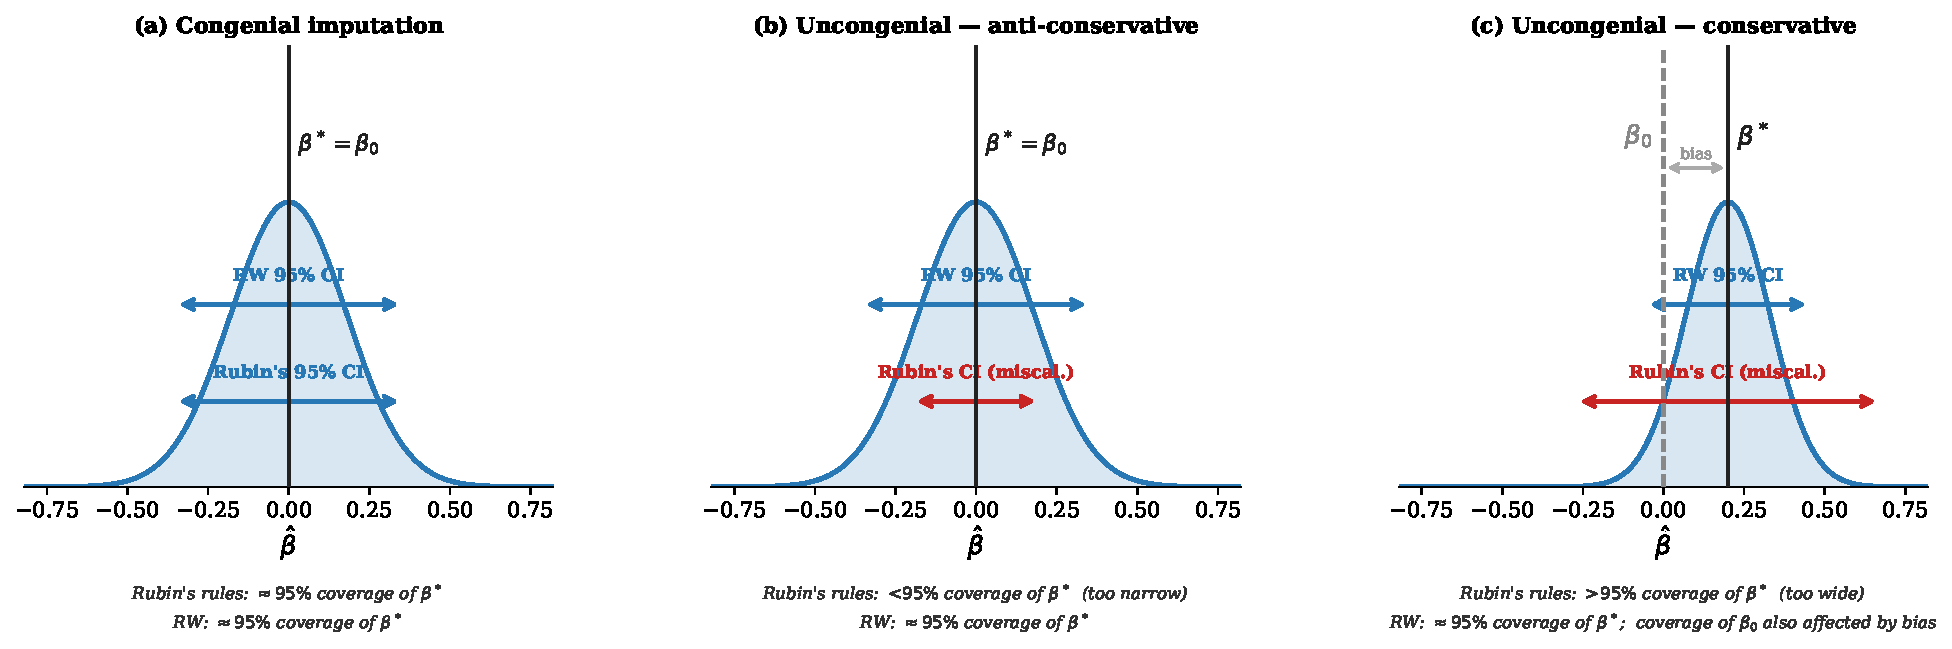
\includegraphics[width=\textwidth]{figures/toy_example.pdf}
  \caption{Conceptual illustration of variance calibration for
  multiply imputed estimators.
  Each panel shows the sampling distribution of \(\hat\beta\) (shaded
  curve) under repeated study replications, the probability limit
  \(\beta^\ast\) (solid vertical line), and, in panel~(c), the
  data-generating coefficient \(\beta_0\) (dashed vertical line).
  Horizontal brackets indicate 95\% confidence intervals from RR (lower bracket, red when miscalibrated) and from the RW
  estimator (upper bracket, blue).
  Panel~(a): congenial imputation, both intervals are correctly
  sized and achieve approximately 95\% coverage of \(\beta^\ast\).
  Panel~(b): uncongenial, anti-conservative case, the RR interval
  is too narrow, leading to under-coverage of \(\beta^\ast\); the RW
  interval is correctly sized.
  Panel~(c): uncongenial, conservative case with estimator bias
  (\(\beta^\ast\ne\beta_0\)), the RR interval is too wide,
  producing over-coverage of \(\beta^\ast\); coverage of \(\beta_0\)
  depends additionally on the bias \(\beta^\ast-\beta_0\).
  The primary simulation diagnostic in
  Section~\ref{simulation-studies} is coverage of \(\beta^\ast\),
  because it isolates variance calibration from point-estimator bias.}
  \label{fig:schematic}
\end{figure}
%======================================================================
% 2.4 Variance estimation using Robins-Wang
%======================================================================
\subsection{Variance estimation using Robins--Wang}
\label{robinswang-variance-components}
\subsubsection{The three sources of variability}
We begin by giving an overview of each component of the Robins--Wang
(RW) variance estimator, and then provide formal definitions.  The
multiply imputed estimator \(\hat\beta\) solves an averaged
complete-data estimating equation, and its repeated-sampling
variability has exactly three first-order sources.
\emph{Source 1: analysis-score variability.}  Even if the
imputation-model parameter \(\psi\) were known exactly and held fixed,
\(\hat\beta\) would still vary across repeated study replications,
because the analysis scores \(U_i(\beta)\) fluctuate with the observed
data.  This is the same variability that ordinary complete-data
sandwich inference would estimate.  It does not vanish as the number of
imputations \(m\) grows, because it reflects between-subject variation
in the analysis, not between-imputation variation.
\emph{Source 2: imputation-parameter uncertainty.}  In practice,
\(\psi\) is estimated from the observed data, and this estimation
uncertainty propagates into \(\hat\beta\) through the imputed values.
The propagation has two steps.  First, \(\hat\psi\) fluctuates around
its limit across replications, with magnitude governed by its influence
function \(d_i\) (Section~\ref{data-notation}).  Second, those
fluctuations shift the imputed values, which in turn shift the analysis
score; how strongly depends on the sensitivity of the analysis score to
the imputation score.  These quantities are defined through the
parametric imputation score; Section~\ref{extension-2} shows how a
smooth donor-selection working law supplies the analogous score for
PMM.
\emph{Source 3: cross-covariance.}  Sources 1 and 2 are not
independent, because the same observed records drive both the analysis
score and the imputation-parameter estimator.  A subject that pushes
\(\hat\psi\) in one direction also tends to shift the analysis score in
a correlated direction.  Ignoring this dependence would misrepresent
the true variance, so a cross-covariance term accounts for it
explicitly.
How does RR compare?  The within-imputation variance is an
estimate of Source 1, and the between-imputation variance is an
approximation of Source 2.  However, their additive combination is
valid only under congeniality.  When the imputation and analysis
procedures are uncongenial, the between-imputation component conflates
Sources 2 and 3 incorrectly: it inflates the variance in settings where
the imputation model uses information beyond the analysis (as in the GS
validation benchmark, where RR was conservative by \(29\%\)), and
deflates it where the analysis exploits structure the imputation model
does not capture (as in the RW missing-data benchmark, where RR is
anti-conservative).  The RW estimator builds all three sources directly
from estimating-equation quantities, which is what makes it valid
without congeniality.  The formal definitions below make these three
sources precise.
\subsubsection{Components of the RW variance estimator}
We first present the RW variance estimator in the setting RW originally
considered, in which all missing values are drawn from a parametric
imputation model indexed by \(\psi\); in
Section~\ref{improved-variance} we extend the RW variance estimator to
chained-equation and PMM imputation.  Beyond the influence function
\(d_i\) of \(\hat\psi\) introduced in Section~\ref{data-notation}, one
further score-type object enters the RW calculation: the missing-value
score \(S_{\mathrm{mis},i}\), the imputation-model score evaluated at
the imputed value for record \(i\).  In sample form the influence
function is
\[
d_i
=
-\Bigl\{P_n\,\partial S_{\mathrm{obs},i}/\partial\psi^\top\Bigr\}^{-1}
S_{\mathrm{obs},i}.
\]
Because \(S_{\mathrm{obs},i}\) is zero for records with nothing observed
for the imputed variable, \(d_i\) is supported only on records that
contribute to the imputation fit, and the sums defining \(\widehat\alpha\)
and \(\widehat C\) below run effectively over those records.
\citet{robins2000inference} express the first-order variance of
\(\hat\beta\) using \(U\), \(S_{\mathrm{mis}}\), and \(d\).  In sample
form, the sandwich variance estimator is
\[
\widehat\Gamma
=
\frac{1}{n}\widehat\tau^{-1}\widehat\Delta\,\bigl(\widehat\tau^{-1}\bigr)^{\!\top},
\qquad
\widehat\Delta
=
\widehat\Omega
+\widehat\kappa\widehat\alpha\widehat\kappa^\top
+\widehat C .
\]
The three matrices inside \(\widehat\Delta\) are empirical second moments
of order one; the leading \(1/n\) converts the sandwich limit for
\(\sqrt n(\hat\beta-\beta^\ast)\) into the finite-sample variance of
\(\hat\beta\).  We keep this scaling explicit so that \(\widehat\Delta\)
is directly comparable with the population formulas in
\citet{robins2000inference}.
The \emph{bread} \(\widehat\tau\) is the average derivative of the
completed-data estimating equation with respect to \(\beta\),
\[
\widehat\tau
=
\frac{1}{nm}\sum_{p=1}^m\sum_{i=1}^n
\left.\frac{\partial U_i^{(p)}(\beta)}{\partial\beta^\top}
\right|_{\beta=\hat\beta}.
\]
It linearises the estimating equation around the solution
\(\hat\beta\), converting the sandwich into units of
\(\mathrm{Var}(\hat\beta)\).  We use \emph{bread} and \emph{meat} in
their standard sandwich-variance sense: \(\widehat\tau\) estimates the
expected derivative of the averaged estimating function, and
\(\widehat\Delta\) estimates the variance of its subject-level
contributions.
As described above, the \emph{meat} \(\widehat\Delta\) is made up of three
components, corresponding to the three sources of variance.  We now give
their explicit forms.
\medskip
\noindent\textit{Source 1: analysis-score covariance.}\enskip
The first piece is the outer product of each subject's
imputation-averaged analysis score \(\bar U_i\).  Averaging over
imputations within each subject eliminates imputation noise, leaving
only the between-subject variation in the analysis score that would
exist even if \(\psi\) were known:
\[
\widehat\Omega
=
\frac{1}{n}\sum_{i=1}^n
\bar U_i(\hat\beta)\,\bar U_i(\hat\beta)^\top.
\]
\medskip
\noindent\textit{Source 2: imputation-parameter uncertainty.}\enskip
The second piece is assembled from two building blocks.  The matrix
\(\widehat\kappa\) measures how sensitively the analysis score responds
to a change in the imputed value: it is the sample cross-moment of the
analysis score \(U_i^{(p)}\) and the missing-value score
\(S_{\mathrm{mis},i}^{(p)}\), which is the gradient of the imputation
log-likelihood with respect to \(\psi\) evaluated at the imputed value.
A large \(\widehat\kappa\) means that small shifts in \(\psi\), and hence in the imputed values, substantially move the analysis score. The matrix \(\widehat\alpha\) is the variance of the influence contribution \(d_i^{(p)}\) across subjects and imputations; it measures
how much \(\hat\psi\) fluctuates as the observed data change.  Together,
\[
\widehat\kappa
=
\frac{1}{nm}\sum_{p=1}^m\sum_{i=1}^n
U_i^{(p)}(\hat\beta)\,S_{\mathrm{mis},i}^{(p)\top},
\qquad
\widehat\alpha
=
\frac{1}{nm}\sum_{p=1}^m\sum_{i=1}^n
d_i^{(p)}d_i^{(p)\top},
\]
and the contribution of imputation-parameter estimation uncertainty to
\(\mathrm{Var}(\hat\beta)\) is \(\widehat\kappa\widehat\alpha\widehat\kappa^\top\).
\medskip
\noindent\textit{Source 3: cross-covariance.}\enskip
The third piece corrects for the dependence between Sources 1 and 2.
Because subject \(i\) simultaneously contributes to \(\bar U_i\) (the
analysis score) and to \(\bar d_i\) (the influence on \(\hat\psi\)),
the two sources are correlated at the individual level.  Writing
\(\bar d_i = m^{-1}\sum_{p=1}^m d_i^{(p)}\) for the
imputation-averaged influence contribution, the cross-covariance is
\[
\widehat C
=
\frac{1}{n}
\Bigl[
\widehat\kappa
\Bigl\{\sum_{i=1}^n \bar d_i\,\bar U_i^\top\Bigr\}
+
\Bigl\{\sum_{i=1}^n \bar U_i\,\bar d_i^\top\Bigr\}
\widehat\kappa^\top
\Bigr]
=
\frac{1}{n}
\bigl[
\widehat\kappa\,\bar d^\top \bar U
+
\bar U^\top\bar d\,\widehat\kappa^\top
\bigr],
\]
where \(\bar U\) and \(\bar d\) are the \(n\times q\) and \(n\times c\)
matrices with rows \(\bar U_i^\top\) and \(\bar d_i^\top\), and
\(c=\dim(\psi)\) as introduced in Section~\ref{data-notation}.  The
symmetrisation (adding the transpose) ensures \(\widehat\Delta\) is
symmetric.  The RR variance estimator implicitly sets a version of this
term to zero, which is one reason it is miscalibrated under
uncongeniality.
% Sec 3: Improved variance estimation (intro + 3.1 MICE [04], 3.2 PMM [05] via internal \input)
\section{Improved variance estimation with multiply-imputed data}
\label{improved-variance}
This section extends the RW framework beyond the parametric imputation
model assumed in Section~\ref{robinswang-variance-components}. For
chained conditional (MICE) imputation, there is no joint imputation
score: \(S_{\mathrm{mis}}\) and \(d\) are replaced by stacked vectors
assembled from each conditional model block, as developed in
Section~\ref{extension-1}; we call the resulting estimator RW-MICE.
For predictive mean matching, the completed value is copied from an
observed donor rather than drawn from a parametric distribution, so
two things change: the donor selection needs a differentiable working
score, and completed rows sharing a donor are not independent
summands, requiring \(\widehat\Omega\) and \(\widehat C\) to be
formed at the donor-source level. This is developed in
Section~\ref{extension-2}, yielding the RW-PMM estimator.
\subsection{RW variance for chained conditional imputation models}
\label{extension-1}
The RW framework of Section~\ref{robinswang-variance-components} requires
three ingredients
tied to a joint parametric imputation likelihood: a parameter vector
\(\psi\) indexing the joint imputation distribution, an observed data
score equation \(\sum_i S_{\mathrm{obs},i}(\psi)=0\) whose solution
defines \(\hat\psi\), and the resulting missing value score
\(S_{\mathrm{mis},i}\) and nuisance influence \(d_i\).  MICE supplies
none of these.  Its conditional working models are fitted block by
block, where a block is a single variable imputed by its own
conditional model (the default in \texttt{mice}) or a group of
variables imputed jointly; the blockwise fits do not correspond to any
joint imputation likelihood, and admit no global parameter solving a
single score equation.  Even if one concatenated the blockwise
parameters as \(\psi = (\psi_1,\ldots,\psi_R)\), where \(R\) denotes
the number of imputation blocks, MICE conditional models are in
general mutually incompatible: they need not correspond to any joint
distribution over the missing variables, so no joint likelihood exists
and no global score equation of the form
\(\sum_i S_{\mathrm{obs},i}(\psi)=0\) can be defined.
Our proposed resolution is to shift from one global estimated parameter
to one realized parameter draw per block per imputation.  In each
imputation \(p\), MICE generates a parameter state \(\psi_r^{(p)}\) for
block \(r\), the coefficient draw used to produce that block's completed
values, and this realized state is already recorded in a standard MICE
run in \texttt{mice}.  We evaluate the RW score and nuisance components
at these realized states, one block at a time, and stack the per-block
contributions into composite vectors that are substituted into the
unchanged RW formula.  No joint imputation likelihood is assumed, and
no modeling choices are required beyond the conditional models that
MICE already fits.
The non-trivial step is justifying that stacking works.  Two conditions
must hold: the realized states \(\psi_r^{(p)}\) must concentrate around
their blockwise working limits \(\psi_{r0}\) fast enough that evaluating
at \(\psi_r^{(p)}\) rather than \(\psi_{r0}\) changes the empirical
moments only at negligible order; and the stacked empirical moments must
consistently estimate the population RW variance components for the MICE
estimator without a coherent joint likelihood.  Both are established in
Appendix~\ref{appendix-theory}; the rest of this section builds the
construction.
\subsubsection{Sequential conditional working law}
Suppose the missing variables are imputed in blocks \(r=1,\ldots,R\).
For block \(r\), let \(H_{r,i}^{(p)}\) denote the predictors and
previously updated variables used by the conditional model in completed
dataset \(p\), with working model
\(f_r\{Y_{r,i}\mid H_{r,i}^{(p)};\psi_r\}\).
Because the conditional models need not be mutually compatible, each
block has its own working parameter \(\psi_r\), whose working value
\(\psi_{r0}\) is defined as the probability limit of the corresponding
conditional estimator, rather than as a coordinate of a global
\(\psi\).  There is one \(\psi_r\) per block and no relationship between
the \(\psi_r\) values across blocks is assumed or needed.
In a proper MICE run, imputation \(p\) draws a parameter state
\(\psi_r^{(p)}\) for each block and generates the completed block from
it.  These realized states are already stored as part of the imputation
output in \texttt{mice}.
We evaluate all RW score components at these realized states
\(\psi_r^{(p)}\).  They are the natural plug-in: already produced by the
MICE run, requiring no additional estimation, and under standard
regularity conditions for proper imputation they concentrate around the
blockwise working limits at rate \(n^{-1/2}\),
\[
\psi_r^{(p)}-\psi_{r0}=O_p(n^{-1/2}).
\]
Because the RW score components are smooth functions of the imputation
parameter, a first-order Taylor expansion shows that evaluating at
\(\psi_r^{(p)}\) rather than \(\psi_{r0}\) changes the empirical RW
moments only at order \(n^{-1/2}\), which is higher order than the
leading term that determines the sandwich limit.  The substitution error
is therefore asymptotically negligible.  The formal statement is in
Appendix~\ref{appendix-theory}.
Next, we describe the score and nuisance objects required for the RW
variance computation.  Write the conditional-model score contribution
for block \(r\), subject \(i\), imputation \(p\) as
\[
s_{r,i}^{(p)}(\psi_r)
=
\frac{\partial}{\partial\psi_r}
\log f_r\{Y_{r,i}\mid H_{r,i}^{(p)};\psi_r\}.
\]
The missing-value score for rows imputed in block \(r\) is the working
score evaluated at the realized state,
\(S_{r,\mathrm{mis},i}^{(p)}=s_{r,i}^{(p)}(\psi_r^{(p)})\); for rows
not imputed in block \(r\), it is zero.  A large score means a small
change in \(\psi_r\) would have moved the imputed value substantially.
The nuisance influence is constructed as follows.  Let \(\delta_{r,i}=1\)
indicate that block \(r\) is observed for subject \(i\), and set
\(S_{r,\mathrm{obs},i}^{(p)}=\delta_{r,i}\,s_{r,i}^{(p)}(\psi_r^{(p)})\).
Define
\[
A_r^{(p)}
=
P_n\!\left\{
\left.
\frac{\partial s_{r,i}^{(p)}(\psi_r)}{\partial\psi_r^\top}
\right|_{\psi_r=\psi_r^{(p)}}
\delta_{r,i}
\right\},
\]
the observed-data Hessian of the block-\(r\) conditional log-likelihood.
The blockwise nuisance influence is the Newton linearization
\[
d_{r,i}^{(p)}
=
-\{A_r^{(p)}\}^{-1}S_{r,\mathrm{obs},i}^{(p)},
\]
the block-\(r\) analogue of the single-model \(d_i\): it measures how
much the block-\(r\) parameter draw would shift if subject \(i\)'s data
changed.  It requires no additional modeling beyond the conditional model
that MICE already fits.  Like the single-model case, \(d_{r,i}^{(p)}\)
is supported only on subjects with block \(r\) observed.
Stacking across all \(R\) blocks then gives the MICE imputation score and
nuisance influence vectors for subject \(i\) in imputation \(p\):
\[
S_{\mathrm{mis},i}^{(p)}
=
\bigl(
S_{1,\mathrm{mis},i}^{(p)\top},\ldots,S_{R,\mathrm{mis},i}^{(p)\top}
\bigr)^\top,
\qquad
d_i^{(p)}
=
\bigl(
d_{1,i}^{(p)\top},\ldots,d_{R,i}^{(p)\top}
\bigr)^\top.
\]
The conditions required of each block are minimal: a regular
observed-score derivative (so that \(A_r^{(p)}\) is invertible), finite
second moments for the score contributions, and a realized state that
concentrates at its working limit.  No coherent joint likelihood across
blocks is needed.
Stacking automatically captures cross-block parameter uncertainty.  The
off-diagonal elements of \(\alpha = E[d_i d_i^\top]\), such as
\(E[d_{r,i}\,d_{r',i}^\top]\) for \(r\neq r'\), reflect correlation
between estimation uncertainty in different blocks, which arises because
the same observed data contribute to both conditional model fits.  These
terms are non-zero in general and are automatically included when
\(\widehat\alpha\) is formed from the full stacked vectors \(d_i^{(p)}\).
\subsubsection{RW components for the MICE estimator}
The analysis estimator is still defined by the averaged completed-data
estimating equation \(0=P_n\bar U(\hat\beta)\).  All RW components are
therefore similar to their Section~\ref{robinswang-variance-components}
counterparts, with the single-model \(S_{\mathrm{mis},i}^{(p)}\) and
\(d_i^{(p)}\) replaced by the stacked MICE quantities defined above; we
call the resulting variance estimator RW-MICE.
Concretely, the bread \(\hat\tau\) is computed exactly as before; the
three covariance pieces are:
\begin{align*}
\widehat\Omega
&=
\frac{1}{n}\sum_{i=1}^n \bar U_i(\hat\beta)\,\bar U_i(\hat\beta)^\top,
\\[4pt]
\widehat\kappa
&=
\frac{1}{nm}\sum_{p=1}^m\sum_{i=1}^n
U_i^{(p)}(\hat\beta)\,S_{\mathrm{mis},i}^{(p)\top},
\qquad
\widehat\alpha
=
\frac{1}{nm}\sum_{p=1}^m\sum_{i=1}^n
d_i^{(p)}d_i^{(p)\top},
\\[4pt]
\widehat C
&=
\frac{1}{n}
\bigl[
\widehat\kappa\,\bar d^\top \bar U
+
\bar U^\top\bar d\,\widehat\kappa^\top
\bigr],
\end{align*}
where \(\bar U\) and \(\bar d\) are the \(n\times q\) and
\(n\times\dim(\psi)\) matrices with rows \(\bar U_i^\top\) and
\(\bar d_i^\top\), and \(\dim(\psi)=\sum_r\dim(\psi_r)\) is the total
number of imputation parameters across all blocks.
Stacking changes the internal block structure of the matrices.
The matrix \(\widehat\kappa = [\widehat\kappa_1,\ldots,\widehat\kappa_R]\)
is block-partitioned by imputation block, with
\(\widehat\kappa_r = (nm)^{-1}\sum_{p,i}U_i^{(p)}S_{r,\mathrm{mis},i}^{(p)\top}\)
measuring how sensitive the analysis score is to block \(r\)'s parameter;
because the analysis equation mixes contributions from all imputed
variables, \(\widehat\kappa_r\) is typically non-zero even for blocks
whose variables do not appear directly in the analysis estimating
function (in parametric regression analysis models, blocks other than
the primary analysis covariate).  The matrix
\(\widehat\alpha\) has \((r,r')\) block
\(\widehat\alpha_{rr'} = (nm)^{-1}\sum_{p,i}d_{r,i}^{(p)}\,d_{r',i}^{(p)\top}\);
the off-diagonal blocks for \(r\neq r'\) capture cross-block parameter
uncertainty and are non-zero whenever subjects contribute to both
conditional model fits.  Dropping them would incorrectly assume
independence of estimation uncertainty across blocks, which fails unless
missing data patterns are block-monotone with no shared covariates.
Consistency of the stacked estimator is established in
Appendix~\ref{appendix-theory}; when \(R=1\) the construction reduces
to the single-model RW estimator of
Section~\ref{robinswang-variance-components}.
The MICE extension requires no new modeling beyond what a standard MICE
run already produces.  Given the completed datasets and the recorded
parameter draws \(\psi_r^{(p)}\), every RW component is computed from
formulas unchanged in form from Section~\ref{robinswang-variance-components}.
The only structural change is that \(S_{\mathrm{mis}}\) and \(d\) are
block vectors, and the resulting sandwich automatically accounts for
within-block and cross-block parameter uncertainty through the full
block structure of \(\widehat\alpha\).
\subsection{RW variance estimation with predictive mean matching}
\label{extension-2}
Predictive mean matching (PMM) is attractive in medical applications
because it imputes plausible observed values rather than unrestricted
model-based draws: the imputed value is not a prediction but a copy of an
actual observed record, which respects distributional constraints that a
parametric draw might violate.  The same feature, however, creates two
problems for the RW variance construction that do not arise in fully
parametric imputation.

The first problem concerns differentiation of the donor-selection rule.
Standard PMM selects
the donor by finding the \(k\) observed records whose predictive mean is
closest to the recipient's predictive mean, the donor pool, and sampling
one uniformly from that pool. This nearest-neighbor rule is a step
function of the imputation parameter \(\psi\): a small shift in \(\psi\)
that does not change the donor pool produces no change in the donor
probabilities, while a shift that just excludes a current neighbor
produces a discontinuous jump. A direct log-gradient of the selected
donor's probability is therefore zero wherever the pool is unchanged
and undefined at a boundary. It does not provide a regular missing-value
score for the RW cross-moment \(\kappa=E\{US_{\mathrm{mis}}^\top\}\).
This difficulty does not prevent calculation of the fitted regression's
influence contributions \(d_i\) or their second moment \(\alpha\).

The second problem is that PMM induces correlation between recipients
that share a donor.  When several missing recipients copy from the same
observed donor, their completed-data analysis scores share a common
stochastic source, the value of the donor record
\citep{rao1992jackknife, chen2002common}.
A random shift in the donor's observed value can affect several
recipient scores simultaneously. The rowwise second moment
\(\sum_i U_i U_i^\top\) does not include cross-products between these
records. Their omission need not always decrease the estimated variance;
the direction depends on the analysis scores.

In this section, we propose an RW estimator that addresses each of
these problems at the specific variance component it affects; we call
this estimator RW-PMM, to contrast with the RW-MICE estimator of
Section~\ref{extension-1}.  Section~\ref{smooth-copied-donor}
defines a differentiable working probability for calculating
\(\widehat\kappa\), without changing the imputations produced by
\texttt{mice}. Section~\ref{donor-source-analysis-scores} aggregates
analysis scores by their recorded donor to construct
\(\widehat\Omega\) and \(\widehat C\). These are working approximations
for variance estimation, not changes to the PMM sampling rule.
\subsubsection{Donor probabilities for variance estimation}
\label{smooth-copied-donor}
Consider one continuous variable \(A\) imputed by PMM, with observed
and missing sets \(\mathcal O_A\) and \(\mathcal M_A\). Let
\(x_i\in\mathbb R^c\) contain the fully observed matching predictors,
including an intercept. Under the default matching rule in \texttt{mice},
observed donors use the fitted regression coefficient
\(\hat\psi^{(p)}\), whereas recipients use a coefficient draw
\(\dot\psi^{(p)}\). Their matching predictions are
\[
a_j^{(p)}=x_j^\top\hat\psi^{(p)},\qquad
t_i^{(p)}=x_i^\top\dot\psi^{(p)}.
\]
Let \(\mathcal N_i^{(p)}\) contain the \(k\) donor predictions closest
to \(t_i^{(p)}\). The actual imputation is unchanged:
\[
P\{J_i^{(p)}=j\mid\text{fitted model and coefficient draw}\}
=\frac{\mathbf 1\{j\in\mathcal N_i^{(p)}\}}{k},
\qquad A_i^{(p)}=A_{J_i^{(p)}}^{\mathrm{obs}}.
\]
The selected donor IDs and completed values are retained exactly.

For the variance calculation, suppress the superscript \(p\) temporarily
and order the \(N=|\mathcal O_A|\) donor predictions as
\(a_{(1)}<\cdots<a_{(N)}\). The following derivatives assume distinct
predictions and a locally unchanged ordering. Donor \((r)\) is among
the \(k\) nearest donors to a scalar prediction \(t\) precisely when
\(\ell_{(r)}<t<u_{(r)}\), apart from ties at the endpoints, where
\[
\ell_{(r)}=
\begin{cases}
-\infty,&r\leq k,\\
(a_{(r-k)}+a_{(r)})/2,&r>k,
\end{cases}
\qquad
u_{(r)}=
\begin{cases}
(a_{(r)}+a_{(r+k)})/2,&r+k\leq N,\\
\infty,&r+k>N.
\end{cases}
\]
These midpoints are the locations at which a competing donor enters or
leaves the nearest \(k\) positions.

Define an auxiliary prediction \(T_i=t_i+s_i Z\), where
\(Z\sim N(0,1)\) and
\[
s_i^2=x_i^\top\Sigma x_i,\qquad \Sigma=\sigma^2 V.
\]
Here \(\sigma\) is the residual standard-deviation draw from the PMM
regression, and \(V\) is its fitted coefficient covariance factor.
For a full-rank unregularized fit,
\(V=(X_{\mathcal O_A}^\top X_{\mathcal O_A})^{-1}\); the implementation
uses the factor from the \texttt{mice} regression fit. Integrating the
uniform top-\(k\) selection rule over this auxiliary normal distribution
gives the working donor probability
\begin{equation}
p_{ij}=\frac{1}{k}
\left\{\Phi\!\left(\frac{u_j-t_i}{s_i}\right)
-\Phi\!\left(\frac{\ell_j-t_i}{s_i}\right)\right\}.
\label{pmm-probability}
\end{equation}
The expression in braces is the probability of entering the donor pool;
division by \(k\) gives the probability of selection. Thus
\(\sum_{j\in\mathcal O_A}p_{ij}=1\). No auxiliary prediction is drawn
when imputing the data, and the recorded donors are not sampled again
from \(p_{ij}\). Equation~\eqref{pmm-probability} is a normal working
approximation for variance estimation, not the conditional sampling
probability of the recorded \texttt{mice} donor. Its smoothing scale is
determined by the fitted regression covariance; no additional bandwidth
is selected to target a particular coverage level.

To differentiate, shift both \(\hat\psi\) and \(\dot\psi\) by the same
vector \(\delta\), holding their difference and \(\Sigma\) fixed. This
allows both donor predictions and the recipient prediction to move.
For finite endpoints, their derivatives are
\[
\dot\ell_{(r)}=(x_{(r-k)}+x_{(r)})/2,\qquad
\dot u_{(r)}=(x_{(r)}+x_{(r+k)})/2.
\]
Writing \(z_{ij}^{u}=(u_j-t_i)/s_i\) and
\(z_{ij}^{\ell}=(\ell_j-t_i)/s_i\), differentiation gives
\begin{equation}
\dot p_{ij}:=\left.\nabla_\delta p_{ij}(\delta)\right|_{\delta=0}
=\frac{\phi(z_{ij}^{u})(\dot u_j-x_i)
-\phi(z_{ij}^{\ell})(\dot\ell_j-x_i)}{k s_i}.
\label{pmm-probability-derivative}
\end{equation}
Terms corresponding to infinite endpoints are zero. The derivatives
sum to zero over donors. An intercept shift moves all predictions
equally, so its derivative is zero; this does not force the derivatives
for the other coefficients to vanish. Holding \(\Sigma\) fixed is part
of the working linearization, not a claim that its estimation adds no
uncertainty.

\subsubsection{Expected analysis scores and the PMM cross-moment}
The RW cross-moment involves the analysis score as well as the
imputation score. Under the working donor law, define
\(S_{ij}=\dot p_{ij}/p_{ij}\) for \(p_{ij}>0\). Let \(G_{ij}^{(p)}\)
be a working expectation of recipient \(i\)'s analysis score when
donor \(j\) is considered. Then
\[
\sum_{j\in\mathcal O_A}p_{ij}^{(p)}G_{ij}^{(p)}S_{ij}^{(p)\top}
=\sum_{j\in\mathcal O_A}G_{ij}^{(p)}\dot p_{ij}^{(p)\top}.
\]
This identity motivates averaging over candidate donors when calculating
the PMM columns of \(\kappa\), rather than multiplying the realized
recipient score by the working score of its selected donor:
\begin{equation}
\widehat\kappa_{\mathrm{PMM}}
=\frac{1}{nm}\sum_{p=1}^m\sum_{i\in\mathcal M_A}
\sum_{j\in\mathcal O_A}G_{ij}^{(p)}\dot p_{ij}^{(p)\top}.
\label{pmm-kappa}
\end{equation}
Only the donor probabilities are differentiated here; the calculation
does not add a term involving \(\partial G_{ij}/\partial\psi\).
The identity is exact under the working law, but its use for imputations
from \texttt{mice} remains an approximation.

To compute \(G_{ij}^{(p)}\), the donor value is integrated under the
fitted normal working model
\(A_j^\dagger\sim N(a_j^{(p)},(\sigma^{(p)})^2)\), rather than fixed
at its observed value. The recipient's own observed covariates are
retained. If a subsequent variable is imputed using \(A\) as a predictor,
its distribution is evaluated at \(A_j^\dagger\) using the recorded
conditional model. In notation,
\[
G_{ij}^{(p)}
=E_{\mathrm{work}}\!\left[
U_i\{A_j^\dagger,Y_i^\dagger;\hat\beta^{(p)}\}
\mid\text{fitted models and recipient's observed covariates}
\right],
\]
where \(Y_i^\dagger\) denotes any such subsequent imputed variable;
observed outcomes are kept fixed. The analysis contribution includes its
original subset indicator. This expectation is used only in
\eqref{pmm-kappa}, not to replace any completed value or the analysis
scores used in donor-source aggregation.

For example, if \(A\) is the response in a linear analysis with fully
observed design vector \(z_i\) and fitted residual variance
\(\hat v^{(p)}\), then
\[
U_i^{(p)}=\frac{z_i\{A_i^{(p)}-z_i^\top\hat\beta^{(p)}\}}{\hat v^{(p)}},
\qquad
G_{ij}^{(p)}=\frac{z_i\{a_j^{(p)}-z_i^\top\hat\beta^{(p)}\}}{\hat v^{(p)}}.
\]
For a logistic analysis of \(D\) on \(A\) restricted to \(A>c_0\), let
\(z(a)=(1,a)^\top\) and
\(\pi_\beta(a)=\expit\{z(a)^\top\beta\}\). Let \(h_i^{(p)}(a)\)
be the probability of \(D_i=1\) under its recorded logistic imputation
model, evaluated at \(A=a\); if \(D_i\) is observed, set
\(h_i^{(p)}(a)=D_i\). The required expectation is
\begin{equation}
G_{ij}^{(p)}=\int_{c_0}^{\infty}
z(a)\{h_i^{(p)}(a)-\pi_{\hat\beta^{(p)}}(a)\}
\frac{1}{\sigma^{(p)}}
\phi\!\left(\frac{a-a_j^{(p)}}{\sigma^{(p)}}\right)\,da.
\label{pmm-binomial-score}
\end{equation}
The integral is not divided by the probability of inclusion: excluded
records contribute zero to the estimating equation normalized by the
full sample size \(n\). It is evaluated numerically using 24-point
Gauss--Legendre quadrature, truncating the standardized normal variable
to \([-10,10]\). Thus the definition of \(G_{ij}\) depends on the
analysis model and any subsequent imputation model, while the donor
probability and its derivative have the same form in both examples.
\subsubsection{Donor-source analysis scores}
\label{donor-source-analysis-scores}
Donor reuse introduces a shared observed value into several completed
records. When recipient \(i_1\)
and recipient \(i_2\) both copy their imputed value from the same observed
donor \(j\), the two completed values are the same observed record
\(A_j^{\mathrm{obs}}\).  Any random variation in \(A_j^{\mathrm{obs}}\) simultaneously affects
the imputed value for \(i_1\) and \(i_2\).  Their analysis scores
\(U_{i_1}^{(p)}\) and \(U_{i_2}^{(p)}\) share the stochastic source
\(A_j^{\mathrm{obs}}\) across repeated samples. This is distinct from
conditional independence of donor draws given a fixed observed dataset.
To represent donor reuse in the variance calculation, each recipient's
analysis score is assigned to its recorded donor.
Let \(U_i^{(p)}(\beta)\) be the completed-data analysis estimating
function contribution for subject \(i\) in imputation \(p\). If recipient
\(i\) copied \(A\) from observed donor \(J_i^{(p)}=j\), then the
stochastic source of the copied \(A\) value is the donor record \(j\).
The donor-source analysis score for observed donor \(j\) is
\[
\widetilde U_j^{(p)}(\beta)
=
U_j^{(p)}(\beta)
+
\sum_{i:J_i^{(p)}=j} U_i^{(p)}(\beta).
\]
The recipient contribution \(U_i^{(p)}(\beta)\) is evaluated using
recipient \(i\)'s completed analysis record; only its stochastic source
is assigned to donor \(j\) for covariance estimation. Rows whose PMM
contribution has been moved to their donor source are set to zero in the
donor-source representation, and rows not involved in the PMM donor map
remain singleton rows. This operation preserves the estimating equation,
\[
\sum_{i=1}^n U_i^{(p)}(\beta)
=
\sum_{i=1}^n \widetilde U_i^{(p)}(\beta),
\]
so the point estimator is unchanged; only the covariance representation
of the first-order analysis scores changes.
This donor-source step is the estimating-equation analogue of the
hot-deck and nearest-neighbor variance idea that an observed donor is the
sampling source for both its own completed record and the recipient
records that copy from it
\citep{rao1992jackknife,chen2002common,kim2004fractional,yang2020pmm}.
If donor \(j\) supplies values for recipients \(i_1,\ldots,i_r\), the
ordinary rowwise meat contains
\[
U_jU_j^\top+\sum_{\ell=1}^r U_{i_\ell}U_{i_\ell}^\top,
\]
whereas the donor-source meat contains
\[
\Bigl(U_j+\sum_{\ell=1}^rU_{i_\ell}\Bigr)
\Bigl(U_j+\sum_{\ell=1}^rU_{i_\ell}\Bigr)^\top .
\]
The second expression includes all cross-products among records sharing
the same observed donor source.  Expanding, the donor-source meat for
donor \(j\) equals the rowwise meat plus the correction terms
\(U_j\sum_\ell U_{i_\ell}^\top + \sum_\ell U_{i_\ell}U_j^\top +
\sum_{\ell\neq\ell'} U_{i_\ell}U_{i_{\ell'}}^\top\): the first two terms
represent donor--recipient cross-products, and the third represents
cross-products among recipients that share
the same donor.  When no recipients copy from donor \(j\) (i.e., donor
\(j\) is only a self-source), the donor-source meat coincides with the
rowwise meat for that record.
The terms \(U_{i_\ell}\) are still the
recipient-specific analysis scores computed from recipient \(i_\ell\)'s
own covariates and eligibility status; the aggregation changes the source of covariance, not the completed-data estimating equation
or any individual record's contribution to the point estimate.
It does not assert that scores assigned to different donors are
independent or that the PMM matching uncertainty is fully described by
this aggregation alone.
\subsubsection{RW components for use with PMM}
For imputation \(p\), let \(U^{(p)}\) be the \(n\times q\) matrix of
rowwise analysis scores evaluated at the completed-data estimate
\(\hat\beta^{(p)}\), and \(\widetilde U^{(p)}\) the corresponding
donor-source matrix. The pooled point estimate remains
\(\hat\beta=m^{-1}\sum_p\hat\beta^{(p)}\). Define
\[
\bar{\widetilde U}
=
\frac{1}{m}\sum_{p=1}^m \widetilde U^{(p)},
\qquad
\widehat\Omega_{\mathrm{src}}
=
P_n\{\bar{\widetilde U}_i
\bar{\widetilde U}_i^\top\},
\]
where \(P_n f_i=n^{-1}\sum_i f_i\). Aggregation is performed using each
imputation's actual donor IDs before averaging over imputations.
The PMM columns of \(\widehat\kappa\) are given by
\eqref{pmm-kappa}. For any additional normal or logistic imputation
models, their columns retain the RW-MICE calculation
\[
\widehat\kappa_{\mathrm{par}}
=
\frac{1}{nm}\sum_{p=1}^m\sum_{i=1}^n
U_i^{(p)}S_{\mathrm{par},i}^{(p)\top}.
\]
These columns and the PMM columns are placed in the same parameter order
as the stacked influence contributions \(d_i^{(p)}\).
For the PMM regression, the observed-score linearization used in the
implementation is
\[
H^{(p)}=-\frac{1}{n(\sigma^{(p)})^2}
\sum_{j\in\mathcal O_A}x_jx_j^\top,\qquad
d_{\mathrm{PMM},i}^{(p)}=
\begin{cases}
-\{H^{(p)}\}^{-1}\dfrac{x_i(A_i-a_i^{(p)})}{(\sigma^{(p)})^2},
&i\in\mathcal O_A,\\[4pt]
0,&i\in\mathcal M_A.
\end{cases}
\]
This contribution describes the fitted matching coefficients, not the
copied donor value. The PMM block has no separate residual-variance
coordinate. Influence contributions for additional normal or logistic
models are calculated as in Section~\ref{extension-1}. With the resulting
stacked vector, define
\[
\widehat\alpha=\frac{1}{nm}\sum_{p=1}^m\sum_{i=1}^n
d_i^{(p)}d_i^{(p)\top},\qquad
\bar d_i=\frac{1}{m}\sum_{p=1}^m d_i^{(p)}.
\]
The donor-source representation is used in \(\widehat\Omega_{\mathrm{src}}\)
and the following cross term, but not in place of the recipient scores
used to calculate \(\widehat\kappa\):
\[
\widehat C_{\mathrm{src}}
=
\widehat\kappa\,P_n\bigl\{\bar d_i\,\bar{\widetilde U}_i^\top\bigr\}
+
P_n\bigl\{\bar{\widetilde U}_i\,\bar d_i^\top\bigr\}\,\widehat\kappa^\top .
\]
The final RW variance estimator for use with PMM is
\[
\widehat\Delta_{\mathrm{PMM}}
=
\widehat\Omega_{\mathrm{src}}
+
\widehat\kappa\,\widehat\alpha\,\widehat\kappa^\top
+
\widehat C_{\mathrm{src}},
\qquad
\widehat\Gamma_{\mathrm{PMM}}
=
\frac{1}{n}
\widehat\tau^{-1}
\widehat\Delta_{\mathrm{PMM}}
\bigl(\widehat\tau^{-1}\bigr)^{\!\top},
\]
where
\[
\widehat\tau=\frac{1}{nm}\sum_{p=1}^m\sum_{i=1}^n
\left.\frac{\partial U_i^{(p)}(\beta)}{\partial\beta^\top}
\right|_{\beta=\hat\beta^{(p)}}.
\]
This construction retains the three-term RW variance form of
Section~\ref{robinswang-variance-components}, while using a working
PMM cross-moment and a donor-source analysis-score representation.
Differentiability of the working probabilities does not by itself
establish consistency for the actual \texttt{mice} PMM procedure.
Its accuracy also depends on the matching approximation and on the
working models used for \(G_{ij}\); these require assessment for the
analysis and imputation settings under consideration.

% Sec 4: Software implementation
\section{Software Implementation}\label{software-implementation}
The variance estimators developed in
Sections~\ref{extension-1}
and~\ref{extension-2}
require objects beyond what the standard output of the
\texttt{mice} package \citep{vanbuuren2011mice} provides.
Specifically, the imputation workflow must expose the per-imputation
parameter draws \(\psi_r^{(p)}\) for each MICE block, the row-level
analysis scores \(U_i^{(p)}\) from each completed-data analysis, and
for PMM-imputed blocks, the donor index \(J_i^{(p)}\) mapping each
recipient to its observed donor.  Algorithm~1 gives the complete
computational workflow; the key constraint is that \(J_i^{(p)}\) and
\(\psi_r^{(p)}\) must be recorded during the imputation phase
and cannot be recovered from completed datasets after the fact.
\begin{algorithm}[RW variance estimation for MICE with optional PMM blocks]
\label{alg:rw-mice-pmm}
\AlgRequire{Observed data $\{O_i\}_{i=1}^n$; conditional imputation models for
blocks $r=1,\ldots,R$; number of imputations $m$; analysis estimating
function $U$; donor pool size $k$ for any PMM-imputed block.}
\AlgEnsure{RW variance estimate $\widehat\Gamma$.}
\AlgState{\textbf{Step 1 (Impute).}}
\AlgFor{$p=1,\ldots,m$}
  \AlgState{\quad For each parametric block $r$: draw
    $\psi_r^{(p)}$ from its large-sample posterior and impute the
    block's missing values; \textbf{record} $\psi_r^{(p)}$.}
  \AlgState{\quad For each PMM block: draw $\psi^{(p)}$, form predictive
    means $\eta_i(\psi^{(p)})$, calibrate the bandwidth $\lambda_i$ by
    the empirical rule to target $k$ effective donors, draw donor
    $J_i^{(p)}$ from the smooth donor law $p_{ij}(\psi^{(p)})$, and copy
    $A_i^{(p)}=A^{\mathrm{obs}}_{J_i^{(p)}}$; \textbf{record}
    $\psi^{(p)}$ and $J_i^{(p)}$.}
\AlgEndFor
\AlgState{\textbf{Step 2 (Analyze).} For each completed dataset, solve the
  complete-data estimating equation; average the solutions to obtain
  $\hat\beta$. Evaluate the row-level scores $U_i^{(p)}(\hat\beta)$ and
  the bread $\widehat\tau$.}
\AlgState{\textbf{Step 3 (Scores).} For each block $r$, evaluate
  $S_{r,\mathrm{mis},i}^{(p)}$ and $d_{r,i}^{(p)}$ at the recorded
  $\psi_r^{(p)}$ (Section~\ref{extension-1}); for a PMM block, evaluate
  $S_{\mathrm{PMM},i}^{(p)}$ (Section~\ref{smooth-copied-donor}) and
  aggregate analysis scores to the donor source,
  $\widetilde U^{(p)}$, using the recorded $J_i^{(p)}$
  (Section~\ref{donor-source-analysis-scores}). Stack across blocks.}
\AlgState{\textbf{Step 4 (Assemble).} Form $\widehat\Omega$ (or
  $\widehat\Omega_{\mathrm{src}}$), $\widehat\kappa$, $\widehat\alpha$,
  $\widehat C$ (or $\widehat C_{\mathrm{src}}$), set
  $\widehat\Delta=\widehat\Omega+\widehat\kappa\widehat\alpha\widehat\kappa^\top+\widehat C$.}
\AlgReturn{$\widehat\Gamma=n^{-1}\widehat\tau^{-1}\widehat\Delta\,\bigl(\widehat\tau^{-1}\bigr)^{\top}$.}
\end{algorithm}
We have developed an \textsf{R} package that is designed to intake a
\texttt{mice} imputation object and return RW variance estimators using
similar syntax to the \texttt{pool} function in \texttt{mice} that
returns RR variance estimators.  The package is available at
\url{https://github.com/LucyMcGowan/rw}.
% Sec 5: Experiments with simulated data
\section{Experiments with simulated data}
\label{simulation-studies}
\subsection{Estimators and evaluation metrics}
\label{sim-estimators}
We compare four variance estimators in two imputation families.  For
chained parametric MICE, RW-MICE denotes our stacked Robins--Wang
estimator (Section~\ref{extension-1}) and RR-MICE the Rubin's-rules
variance applied to the same imputations.  For predictive mean matching,
RW-PMM denotes the Robins--Wang estimator for use with PMM
(Section~\ref{extension-2}) and RR-PMM the Rubin's-rules variance
applied to the PMM imputations.  Within each RW/RR pair the point
estimator \(\hat\beta\) is identical; only the variance estimator
differs.
The two simulation settings are chosen to stress-test the two extensions
developed in Sections~\ref{extension-1}
and~\ref{extension-2} in
qualitatively different ways.
The first setting, the missing-data benchmark of \citet{robins2000inference},
uses ordinary outcome missingness and a linear analysis estimating equation.
Because the data-generating mechanism is well understood, we know in advance
which direction RR should fail: anti-conservative when the analysis
exploits heteroskedastic structure that the imputation model does not reflect
(panel~(b) of Figure~\ref{fig:schematic}), and conservative when the
imputation model is richer than the analysis (panel~(c)).  This allows the RW-MICE
extension to be evaluated against a known calibration benchmark rather than against
empirical performance alone.  The benchmark also includes PMM variants, which
assess whether the smooth copied-donor correction introduces any artefact under
ordinary missingness.
The second setting, the EHR validation setting of \citet{giganti2020multiple},
is a more demanding test that combines both extensions simultaneously.  Two
variables are imputed by MICE, one continuous and one binary.  The continuous
variable is imputed by either a Gaussian parametric model or by PMM; the binary
variable is imputed by a logistic conditional model.  Critically, the imputed
continuous variable determines both the analysis covariate and the eligibility
criterion for the analysis subset.  This imputation structure is
the canonical case of conservative uncongeniality: the imputation model is
fitted on all subjects, but the analysis equation is evaluated in a subset
whose membership fluctuates with the imputed values, inflating the
between-imputation variance for Rubin's rules.
For each simulation scenario, \(\beta^\ast\) denotes the large-sample target
of the implemented imputation-and-analysis procedure; in finite
simulation summaries it is approximated by the Monte Carlo mean of the
multiply imputed analysis estimator.  The primary variance calibration
measure is coverage of \(\beta^\ast\): for each replicate,
the usual confidence interval \(\hat\beta\pm1.96\widehat{SE}\) is
checked for coverage of \(\beta^\ast\).  This isolates variance
calibration from finite-sample bias.  We also report coverage of the
data-generating coefficient \(\beta_0\), mean bias
\(\hat\beta-\beta_0\), the empirical standard deviation of the Monte
Carlo estimates, and the mean estimated standard error.
Thus, coverage of \(\beta^\ast\)
answers whether the standard error estimates the sampling variability of
the implemented estimator, whereas coverage of \(\beta_0\) also reflects
finite-sample bias and target mismatch.  All simulations use 2500 Monte
Carlo replications per cell.
\subsection{Missing-data benchmark}
\label{simulation-rw-setting}
The missing-data benchmark follows the original simulation structure
used by RW: a hypothetical example involving children at a daycare
center.  Each subject has a group indicator \(A\), an
age covariate \(X\), and a continuous outcome \(Z\).
We use \(A=0\) for infants and \(A=1\) for toddlers, with
\(P(A=1)=1/3\).  Infants have \(X\sim U(0.1,0.8)\) and toddlers have
\(X\sim U(0.8,2.0)\).  In the main variants,
\[
  Z=X+\varepsilon,\qquad
  \varepsilon\mid X,A\sim N\{0,X^{\eta_A}\}.
\]
The outcome is fully observed for infants.  Among toddlers, \(Z\) is
missing with probability 0.60 except in the outcome-dependent
observation variant, where \(V=1\) denotes that \(Z\) is observed.  The
completed-data analysis is the no-intercept least-squares estimating
equation for the coefficient of \(X\) in \(E(Z\mid X)=\beta X\).  In
one variant the analysis is restricted to toddlers; otherwise all
subjects are included.  We generated data with both \(n=150\), matching
the original RW simulations exactly, and \(n=1000\).
The six scenarios are:
\[
\begin{array}{ll}
\text{S1:}  & \eta_0=\eta_1=0,\ \text{analysis restricted to toddlers};\\
\text{S2a:} & \eta_0=\eta_1=1,\ \text{all-subject analysis};\\
\text{S2b:} & \eta_0=\eta_1=-1,\ \text{all-subject analysis};\\
\text{S2c:} & \eta_0=2,\ \eta_1=1,\ \text{all-subject analysis};\\
\text{S3a:} & \eta_0=\eta_1=0,\ P(V=1\mid Z,A=1)=\expit(2-0.5Z);\\
\text{S3b:} & Z=X+0.5X^2+\varepsilon,\ \eta_0=\eta_1=0.
\end{array}
\]
S1 is the subgroup analysis case.  S2a--S2c retain the linear mean
analysis but change the variance relationship between the imputation
and analysis estimating equations.  S3a changes the observation
mechanism among toddlers, and S3b changes the outcome mean while
retaining the linear analysis.  In S3a and S3b, coverage of
\(\beta_0\) can differ from coverage of \(\beta^\ast\) because the
finite-sample estimator is centered away from the data-generating
coefficient.
Tables~\ref{tab:rw-benchmark-n150} and
\ref{tab:rw-benchmark-n1000} summarize the missing-data benchmark by
scenario.
For parametric MICE, RW/RR pairs compare RW-MICE with
RR-MICE.  For PMM, RW/RR pairs compare RW-PMM with
RR-PMM, using donor pool size \(k=5\).  RW-MICE has
coverage of \(\beta^\ast\) close to nominal in both sample size
settings.  RW-PMM shows the same pattern at \(n=1000\), with
coverage of \(\beta^\ast\) between 0.945 and 0.965 across the six
scenarios.  The \(n=150\) PMM cells are more variable, as expected for
small samples with copied donor values, but still correct the most
anti-conservative RR-PMM cells in S1, S2a, S2c, and S3b.  RR can be far from nominal: anti-conservative in S2a and S2c, and
conservative in S2b.  These results reproduce the key RW message in a
chained-equation implementation: when imputation and analysis
estimating equations are uncongenial, variance calibration depends on
the estimating-equation structure rather than on RR alone.

\begin{table}[ht]
\centering
\scriptsize
\setlength{\tabcolsep}{3.5pt}
\begin{tabular}{llrrrrrrr}
\toprule
Scenario & \makecell{Imputation\\model} & \makecell{Mean\\estimate} & Bias &
\makecell{Empirical\\SD} &
\makecell{Mean estimated SE\\RW/RR} &
\makecell{Coverage \(\beta^\ast\)\\RW/RR} &
\makecell{Coverage \(\beta_0\)\\RW/RR} & \makecell{Median corr.\\(score comp.)}\\
\midrule
S1  & Parametric MICE & 0.999 & -0.001 & 0.109 & 0.095 / 0.101 & 0.936 / 0.948 & 0.936 / 0.948 &\\
\addlinespace[1pt]
    & PMM (\(k=5\)) & 0.981 & -0.019 & 0.174 & 0.234 / 0.124 & 0.925 / 0.832 & 0.920 / 0.832 &\\
\addlinespace[1pt]
S2a & Parametric MICE & 0.998 & -0.002 & 0.108 & 0.095 / 0.066 & 0.942 / 0.806 & 0.943 / 0.804 &\\
\addlinespace[1pt]
    & PMM (\(k=5\)) & 0.990 & -0.010 & 0.164 & 0.182 / 0.104 & 0.926 / 0.783 & 0.925 / 0.778 &\\
\addlinespace[1pt]
S2b & Parametric MICE & 0.999 & -0.001 & 0.089 & 0.079 / 0.137 & 0.947 / 0.998 & 0.947 / 0.998 &\\
\addlinespace[1pt]
    & PMM (\(k=5\)) & 0.968 & -0.032 & 0.124 & 0.308 / 0.153 & 0.970 / 0.985 & 0.972 / 0.987 &\\
\addlinespace[1pt]
S2c & Parametric MICE & 0.998 & -0.002 & 0.107 & 0.094 / 0.055 & 0.945 / 0.722 & 0.945 / 0.718 &\\
\addlinespace[1pt]
    & PMM (\(k=5\)) & 0.992 & -0.008 & 0.168 & 0.165 / 0.097 & 0.913 / 0.736 & 0.916 / 0.731 &\\
\addlinespace[1pt]
S3a & Parametric MICE & 0.938 & -0.062 & 0.070 & 0.061 / 0.063 & 0.943 / 0.955 & 0.735 / 0.755 &\\
\addlinespace[1pt]
    & PMM (\(k=5\)) & 0.939 & -0.061 & 0.098 & 0.106 / 0.095 & 0.945 / 0.941 & 0.909 / 0.890 &\\
\addlinespace[1pt]
S3b & Parametric MICE & 1.670 & 0.670  & 0.097 & 0.085 / 0.086 & 0.944 / 0.941 & 0.002 / 0.002 &\\
\addlinespace[1pt]
    & PMM (\(k=5\)) & 1.667 & 0.667 & 0.147 & 0.140 / 0.109 & 0.931 / 0.858 & 0.012 / 0.002 &\\
\bottomrule
\end{tabular}
\caption{Missing-data benchmark at \(n=150\) and \(m=20\), with 2500
Monte Carlo replications per scenario.  Bias is the Monte Carlo mean
estimate minus the data-generating coefficient.  RW/RR pairs
refer to RW-MICE/RR-MICE for parametric MICE rows and
RW-PMM/RR-PMM for PMM rows.}
\label{tab:rw-benchmark-n150}
\end{table}

\begin{table}[ht]
\centering
\scriptsize
\setlength{\tabcolsep}{3.5pt}
\begin{tabular}{llrrrrrrr}
\toprule
Scenario & \makecell{Imputation\\model} & \makecell{Mean\\estimate} & Bias &
\makecell{Empirical\\SD} &
\makecell{Mean estimated SE\\RW/RR} &
\makecell{Coverage \(\beta^\ast\)\\RW/RR} &
\makecell{Coverage \(\beta_0\)\\RW/RR} & \makecell{Median corr.\\(score comp.)}\\
\midrule
S1  & Parametric MICE & 1.000 & -0.000 & 0.059 & 0.059 / 0.060 & 0.950 / 0.952 & 0.950 / 0.953 &\\
\addlinespace[1pt]
    & PMM (\(k=5\)) & 0.996 & -0.004 & 0.063 & 0.065 / 0.047 & 0.948 / 0.859 & 0.949 / 0.860 &\\
\addlinespace[1pt]
S2a & Parametric MICE & 0.999 & -0.001 & 0.059 & 0.060 / 0.040 & 0.952 / 0.812 & 0.952 / 0.810 &\\
\addlinespace[1pt]
    & PMM (\(k=5\)) & 1.000 & 0.000 & 0.065 & 0.065 / 0.041 & 0.952 / 0.784 & 0.952 / 0.785 &\\
\addlinespace[1pt]
S2b & Parametric MICE & 0.999 & -0.001 & 0.045 & 0.046 / 0.082 & 0.950 / 1.000 & 0.951 / 1.000 &\\
\addlinespace[1pt]
    & PMM (\(k=5\)) & 0.996 & -0.004 & 0.046 & 0.053 / 0.055 & 0.965 / 0.982 & 0.965 / 0.982 &\\
\addlinespace[1pt]
S2c & Parametric MICE & 0.999 & -0.001 & 0.059 & 0.059 / 0.034 & 0.955 / 0.725 & 0.953 / 0.726 &\\
\addlinespace[1pt]
    & PMM (\(k=5\)) & 0.999 & -0.001 & 0.064 & 0.064 / 0.039 & 0.945 / 0.762 & 0.945 / 0.760 &\\
\addlinespace[1pt]
S3a & Parametric MICE & 0.939 & -0.061 & 0.038 & 0.038 / 0.038 & 0.949 / 0.954 & 0.626 / 0.645 &\\
\addlinespace[1pt]
    & PMM (\(k=5\)) & 0.939 & -0.061 & 0.038 & 0.039 / 0.037 & 0.954 / 0.941 & 0.658 / 0.618 &\\
\addlinespace[1pt]
S3b & Parametric MICE & 1.672 & 0.672  & 0.052 & 0.052 / 0.052 & 0.953 / 0.945 & 0.000 / 0.000 &\\
\addlinespace[1pt]
    & PMM (\(k=5\)) & 1.688 & 0.688 & 0.054 & 0.055 / 0.042 & 0.954 / 0.868 & 0.000 / 0.000 &\\
\bottomrule
\end{tabular}
\caption{Missing-data benchmark at \(n=1000\) and \(m=50\), with 2500
Monte Carlo replications per scenario.  Columns are defined as in
Table~\ref{tab:rw-benchmark-n150}.}
\label{tab:rw-benchmark-n1000}
\end{table}

These results confirm that the MICE stacking construction
of Section~\ref{extension-1}
correctly captures the three RW variance sources under chained conditional
imputation.  Second, the RW-PMM estimator inherits this
calibration at \(n=1000\) and makes substantial improvements over
RR-PMM even at \(n=150\), where small sample variance is larger.  Both
estimators correctly distinguish between coverage of \(\beta^\ast\) (a
pure variance diagnostic, near-nominal for the proposed methods) and
coverage of \(\beta_0\) (which also reflects the bias of the implemented
estimator, and is low when \(\beta^\ast \neq \beta_0\) as in S3a and S3b).
The benchmark setting, however, does not fully stress test the PMM
correction.  The analysis subset does not depend on the imputed variable:
whether \(Z\) is large or small does not change which subjects enter the
least-squares estimating equation.  The donor-source correlation
adjustment (Section~\ref{donor-source-analysis-scores}) therefore has
limited impact in this setting, because the analysis-score contributions
of recipients with a common donor are not strongly correlated through a
shared eligibility event.  The GS validation setting below provides the
harder test, where the copied donor value simultaneously appears in the
analysis as a covariate and determines the analysis subset.
\clearpage
\subsection{Measurement-error validation setting}
\label{simulation-gs-setting}
The second simulation setting follows the GS electronic health record
validation example \citep{giganti2020multiple}.  The goal is to
estimate the association between a
continuous exposure \(A\) and a binary outcome \(D\).  Only error-prone
versions \(A^\ast\) and \(D^\ast\) are available for every subject, while
the validated variables \(A\) and \(D\) are observed in a validation
subset; the validated values are imputed for the remaining subjects.
The analysis model is a logistic regression of \(D\) on \(A\), restricted
to the post-imputation analysis set \(\{A>2\}\); the eligibility rule
reflects the common situation in which the study question concerns only
subjects above a clinical threshold on the (error-prone, then imputed)
exposure.  We generated data with \(n=2000\) and \(n=4000\), the latter matching the original GS implementation; the full sample-size grid \(n\in\{2000,4000,6000,8000\}\) for parametric MICE is shown in
Figure~\ref{fig:gs-parametric-full-supp}.
This setting is more demanding than the RW benchmark in three concrete
ways. First, there are two MICE blocks, one continuous and one binary,
so the stacking must handle a mixed-model chained structure with
cross-block nuisance terms as in
Section~\ref{extension-1}. Second, the eligibility rule \(\{A>2\}\)
means that the imputed \(A\) value determines whether a subject's
analysis score is zero or nonzero: two recipients copying from the same
donor therefore have correlated eligibility decisions and correlated
analysis score values, making this the setting where the donor source
adjustment of Section~\ref{donor-source-analysis-scores} matters most.
Third, the imputation model is fitted on all subjects while the analysis
runs only in the post imputation subset \(\{A>2\}\), the canonical
case of conservative uncongeniality, which inflates the between-imputation
variance through random subset membership, reproducing the panel~(c)
pattern of Figure~\ref{fig:schematic}.
As in the previous section, we implement both parametric and PMM
imputation.  In the parametric MICE cells, \(A\) is imputed from a Gaussian
conditional working model with predictors \(X_1,X_2,A^\ast,D^\ast\),
and \(D\) from a logistic model with the same predictors plus the
completed \(A\). In the PMM cells, only the continuous \(A\) block is
replaced by the smooth copied donor law; the \(D\) block remains
logistic. This design isolates the PMM correction: the binary block
contributes through the standard RW-MICE framework, while the donor source
adjustment applies only to the \(A\) block that directly drives eligibility.
Tables~\ref{tab:gs-validation-n2000} and
\ref{tab:gs-validation-n4000} report results separately by sample size.
Each table uses the same layout and presents three imputation models:
parametric MICE, PMM with \(k=5\), and PMM with \(k=10\).  We vary the
number of imputations \(m\in\{5,25,50,100\}\) to assess sensitivity to
the number of imputations, and the donor pool size \(k\) because it
governs how widely the smooth law spreads probability over donors;
Results for the larger donor pools \(k=20\) and \(k=30\) are reported
in Appendix~\ref{appendix-simulation-figures}
(Table~\ref{tab:pmm-k-sensitivity-supp};
Figure~\ref{fig:gs-pmm-current-n2000-supp}) and are broadly similar to
those for \(k=5\) and \(k=10\); results across sample sizes for
\(k=5\) are shown in Figure~\ref{fig:gs-pmm-current-k5-supp}.

\begin{table}[!htbp]
\centering
\scriptsize
\setlength{\tabcolsep}{2.5pt}
\begin{tabular}{rlrrrrrrr}
\toprule
\(m\) & \makecell{Imputation\\model} &
\makecell{Mean\\estimate} & Bias &
\makecell{Empirical\\SD} &
\makecell{Mean estimated SE\\RW/RR} &
\makecell{Coverage \(\beta^\ast\)\\RW/RR} &
\makecell{Coverage \(\beta_0\)\\RW/RR} & \makecell{Median corr.\\(score comp.)}\\
\midrule
5   & Parametric MICE & 0.850 & -0.040 & 0.120 & 0.114 / 0.166 & 0.937 / 0.985 & 0.900 / 0.973 &\\
5   & PMM (\(k=5\))  & 0.851 & -0.041 & 0.134 & 0.177 / 0.168 & 0.979 / 0.976 & 0.968 / 0.966 &\\
5   & PMM (\(k=10\)) & 0.842 & -0.046 & 0.136 & 0.149 / 0.169 & 0.956 / 0.978 & 0.944 / 0.962 &\\
\addlinespace[2pt]
25  & Parametric MICE & 0.850 & -0.040 & 0.109 & 0.107 / 0.162 & 0.944 / 0.996 & 0.910 / 0.985 &\\
25  & PMM (\(k=5\))  & 0.854 & -0.037 & 0.125 & 0.136 / 0.165 & 0.963 / 0.991 & 0.947 / 0.978 &\\
25  & PMM (\(k=10\)) & 0.843 & -0.048 & 0.127 & 0.129 / 0.166 & 0.956 / 0.989 & 0.923 / 0.973 &\\
\addlinespace[2pt]
50  & Parametric MICE & 0.850 & -0.040 & 0.108 & 0.107 / 0.162 & 0.946 / 0.998 & 0.907 / 0.984 &\\
50  & PMM (\(k=5\))  & 0.855 & -0.038 & 0.124 & 0.130 / 0.164 & 0.957 / 0.992 & 0.934 / 0.977 &\\
50  & PMM (\(k=10\)) & 0.843 & -0.048 & 0.125 & 0.126 / 0.165 & 0.946 / 0.989 & 0.929 / 0.978 &\\
\addlinespace[2pt]
100 & Parametric MICE & 0.850 & -0.040 & 0.107 & 0.106 / 0.162 & 0.944 / 0.998 & 0.909 / 0.986 &\\
100 & PMM (\(k=5\))  & 0.849 & -0.040 & 0.123 & 0.127 / 0.164 & 0.954 / 0.992 & 0.940 / 0.979 &\\
100 & PMM (\(k=10\)) & 0.843 & -0.048 & 0.124 & 0.124 / 0.165 & 0.953 / 0.991 & 0.934 / 0.986 &\\
\bottomrule
\end{tabular}
\caption{Measurement-error validation setting at \(n=2000\), with 2500
Monte Carlo replications per completed cell.  RW/RR pairs refer
to RW-MICE/RR-MICE for parametric MICE rows and
RW-PMM/RR-PMM for PMM rows.}
\label{tab:gs-validation-n2000}
\end{table}

\begin{table}[!htbp]
\centering
\scriptsize
\setlength{\tabcolsep}{2.5pt}
\begin{tabular}{rlrrrrrrr}
\toprule
\(m\) & \makecell{Imputation\\model} &
\makecell{Mean\\estimate} & Bias &
\makecell{Empirical\\SD} &
\makecell{Mean estimated SE\\RW/RR} &
\makecell{Coverage \(\beta^\ast\)\\RW/RR} &
\makecell{Coverage \(\beta_0\)\\RW/RR} & \makecell{Median corr.\\(score comp.)}\\
\midrule
5   & Parametric MICE & 0.869 & -0.020 & 0.083 & 0.082 / 0.117 & 0.944 / 0.989 & 0.921 / 0.980 &\\
5   & PMM (\(k=5\))  &       &        &       &               &               &               &\\
5   & PMM (\(k=10\)) &       &        &       &               &               &               &\\
\addlinespace[2pt]
25  & Parametric MICE & 0.869 & -0.021 & 0.076 & 0.078 / 0.115 & 0.951 / 0.996 & 0.920 / 0.992 &\\
25  & PMM (\(k=5\))  &       &        &       &               &               &               &\\
25  & PMM (\(k=10\)) &       &        &       &               &               &               &\\
\addlinespace[2pt]
50  & Parametric MICE & 0.869 & -0.021 & 0.075 & 0.077 / 0.115 & 0.950 / 0.995 & 0.920 / 0.992 &\\
50  & PMM (\(k=5\))  &       &        &       &               &               &               &\\
50  & PMM (\(k=10\)) &       &        &       &               &               &               &\\
\addlinespace[2pt]
100 & Parametric MICE & 0.869 & -0.021 & 0.075 & 0.077 / 0.114 & 0.956 / 0.997 & 0.925 / 0.992 &\\
100 & PMM (\(k=5\))  &       &        &       &               &               &               &\\
100 & PMM (\(k=10\)) &       &        &       &               &               &               &\\
\bottomrule
\end{tabular}
\caption{Measurement-error validation setting at \(n=4000\), with 2500
Monte Carlo replications per completed cell.  Columns are defined as in
Table~\ref{tab:gs-validation-n2000}.}
\label{tab:gs-validation-n4000}
\end{table}

\FloatBarrier
Tables~\ref{tab:gs-validation-n2000} and
\ref{tab:gs-validation-n4000} show that RW-MICE tracks the empirical
standard deviation more closely than RR in the parametric
MICE rows across all values of \(m\), confirming that the MICE
extension handles the conservative uncongeniality of this setting.
RR consistently overstates the standard error by
approximately 30--50\%, reproducing the GS finding at these larger
sample sizes (Figure~\ref{fig:gs-parametric}).
For PMM, the empirical rule concentrates the smooth law's probability
on approximately \(k\) donors while assigning positive probability to
the remainder; larger \(k\) spreads probability over more distant
donors. For the completed \(n=2000\) PMM rows,
RW-PMM standard errors are close to the empirical standard
deviation for \(m\ge 25\), while RR is conservative for
the same PMM point estimator.
Across the reported \(n=2000\) PMM validation cells with
\(k\in\{5,10,20,30\}\), coverage of \(\beta^\ast\) for RW-PMM ranges
from 0.943 to 0.979, compared with 0.976 to 0.992 for RR-PMM.  Coverage
of \(\beta_0\) is more sensitive to \(k\) because larger donor pools
admit more distant donors (a wider \emph{donor width}, i.e.\ the spread
of predictive means among eligible donors), which shifts the PMM point
estimator away from \(\beta_0\); this reflects donor-width bias rather
than variance miscalibration.  Results for the larger donor pools
\(k=20\) and \(k=30\) are reported in
Appendix~\ref{appendix-simulation-figures} and are broadly similar to
those for \(k=5\) and \(k=10\).
\subsection{Summary}
Across both settings the proposed RW estimators achieve near-nominal
coverage of \(\beta^\ast\) in most cases, while RR fails in
predictable directions: anti-conservative when the analysis exploits
structure the imputation model does not reflect, and conservative when
the imputation model uses information beyond the analysis. These failures are not
small: they reach 14--23 coverage-point shortfalls in the
anti-conservative direction (RW benchmark, S2a, S2c, S3b) and
approximately 30--50\% SE inflation in the conservative direction (GS
validation setting). The RW-PMM estimator inherits the
calibration of RW-MICE in the benchmark setting and correctly handles
the eligibility-by-imputation correlation structure in the GS setting,
with coverage of \(\beta^\ast\) between 0.943 and 0.979 across the
completed PMM cells. The distinction between coverage of \(\beta^\ast\)
and coverage of \(\beta_0\), illustrated in
Figure~\ref{fig:schematic} and maintained throughout the simulation
tables, is important: when the implemented estimator is biased for
\(\beta_0\) (as in S3a, S3b, and the GS validation setting), coverage
of \(\beta^\ast\) is the correct measure of variance calibration, and
the proposed RW methods achieve it.

\begin{figure}[ht]
\centering
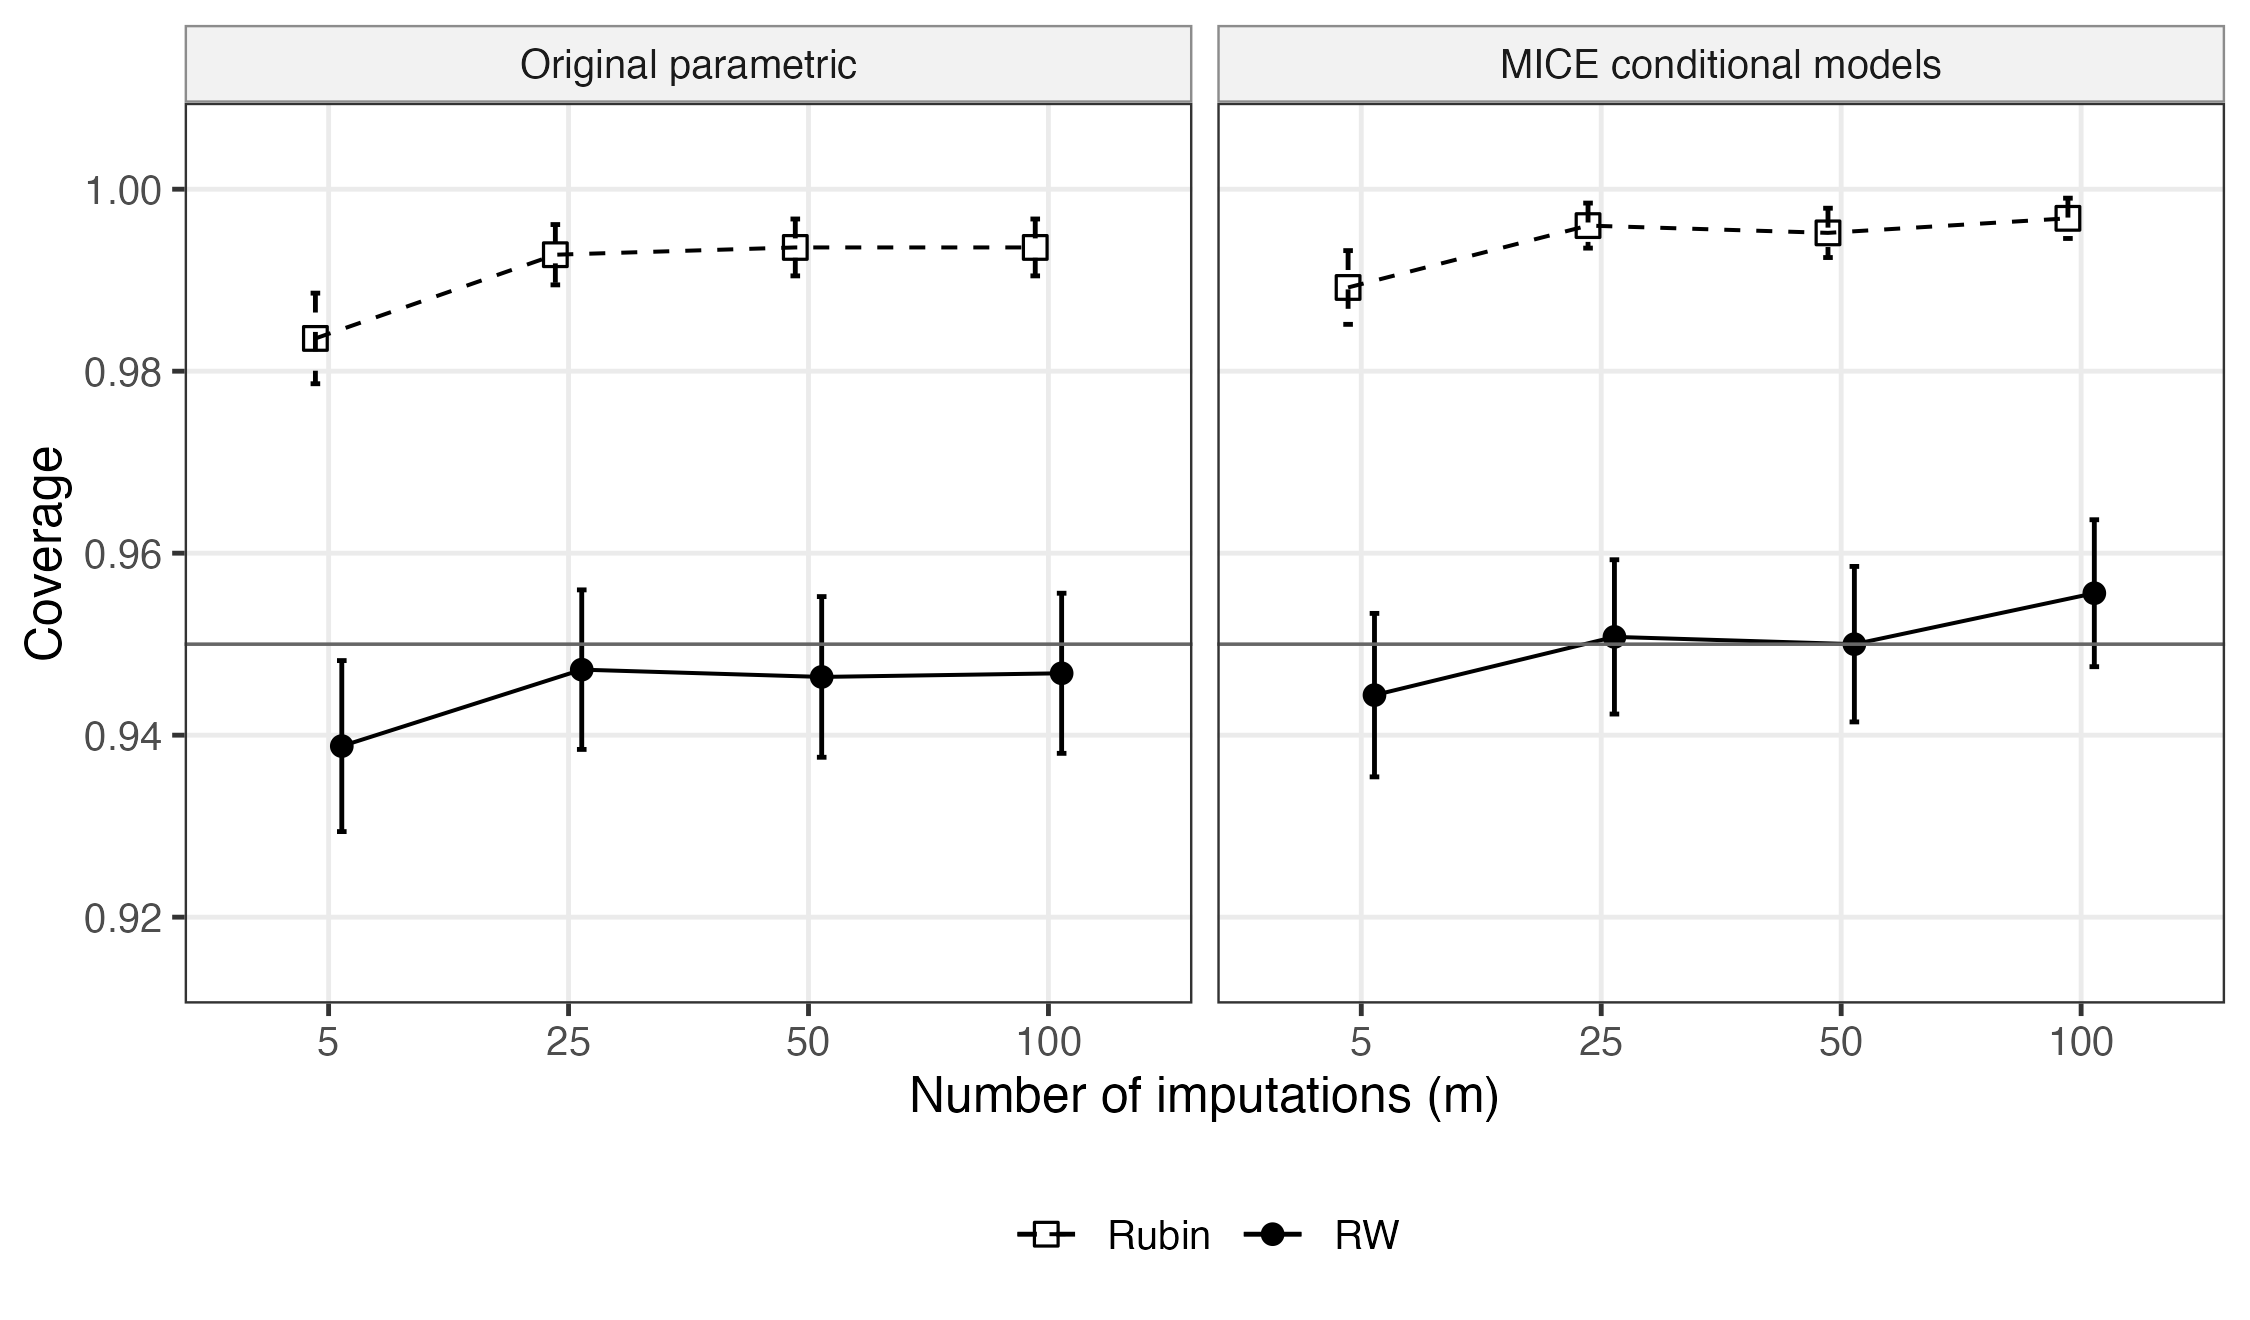
\includegraphics[width=\textwidth]{figures/gs_parametric_coverage_n4000.png}
\caption{Empirical-centered coverage in the Giganti--Shepherd
measurement-error setting with parametric imputation at \(n=4000\).
The left panel shows the original Giganti--Shepherd parametric
implementation, and the right panel shows the chained conditional MICE
implementation.}
\label{fig:gs-parametric}
\end{figure}

\clearpage

% Sec 6: Discussion (Conclusions + Limitations folded in)
\section{Discussion}\label{discussion}
This paper develops two extensions of the estimating-equation variance
framework of \citet{robins2000inference} to settings that arise
routinely in modern medical data
analysis: chained conditional (MICE) imputation and predictive mean
matching.  The extensions are not ad hoc adjustments but follow directly
from the RW construction once the relevant score and nuisance objects are
identified for each setting.  Both extensions are validated in simulation
and the key implementation objects are exposed by a companion \textsf{R}
package, \texttt{rw}, that seamlessly integrates with \texttt{mice}
package output.  Our open-source software is easy to use because it
mirrors the functions already in place for Rubin's rules variance
estimators and takes as input a \texttt{mice} package imputed dataset.
The failure of Rubin's rules under uncongeniality has been understood
since \citet{meng1994multiple} and formalised for estimating equation
analyses by \citet{wang1998large}.  The present work bridges these
theoretical results and applied practice by showing that both failure
modes (anti-conservative and conservative) arise in common MICE
and PMM workflows and can be corrected within the same sandwich
framework.  The GS validation setting, where eligibility is determined
by the imputed variable and Rubin's rules overstate the variance by
approximately 30--50\%, is an instance of Meng's conservative
uncongeniality that has become increasingly common in EHR based analyses
with imputed inclusion criteria \citep{shen2026missingness}.  The
RW-MICE and RW-PMM estimators restore calibration in this setting
without requiring any change to the imputation or analysis workflow.
\paragraph{The bootstrap.}
As noted in Section~\ref{introduction}, the bootstrap is an alternative
to analytic variance estimation under uncongeniality: re-running the
full imputation and analysis procedure across bootstrap samples
consistently estimates the variance of the implemented estimator
regardless of congeniality
\citep{schomaker2018bootstrap, bartlett2020bootstrap}.  The RW estimator
has a practical advantage when the imputation workflow is expensive to
repeat.
\paragraph{Limitations.}
Several limitations should be noted.  First, the PMM extension requires
donor indices \(J_i^{(p)}\) to be recorded during imputation; they
cannot be reconstructed from completed datasets.  This is a software
requirement rather than a theoretical obstacle, and the companion package
handles it automatically, but practitioners using standard
\texttt{mice} output will need to update their imputation workflow.
Second, the present work considers the case where one continuous
variable is imputed by the smooth copied donor law and the remaining
blocks are parametric.  When several variables are imputed by PMM with
potentially different donor maps, the multi-source covariance structure
requires additional work.  The analysis score contributions of two
recipients can be correlated through two independent donor maps
simultaneously, and stacking the donor source representations from
different PMM blocks does not automatically account for this joint
dependence.  Possible extensions include block PMM with common donors or
a multi-way source aggregation; these fit within the same
source-aggregation framework, and we plan to support general PMM
problems in a future release of the package.
Third, the smooth copied donor law is a working device for computing the
RW score; it does not change the imputed values.  The asymptotic
equivalence between the RW estimator for the smooth law and the
bootstrap variance of the hard nearest-neighbor PMM estimator has not
been formally established.  The simulation evidence is supportive, but a
rigorous analysis of the approximation error as \(k\to\infty\) or
\(\lambda\to\infty\) remains an open problem.
Fourth, the paper focuses on Gaussian and logistic analysis estimating
equations.  Extensions to survival analysis, competing risks, or
semiparametric models with partially observed outcomes are not
considered, though the RW framework is in principle applicable to any
regular estimating equation.

\section*{Acknowledgments}
This manuscript was supported in part by the U.S. National Institutes of Health (NIH) grant R37 AI131771 (BDW) and XX (LDM).

\section*{Code availability}
We provide code to reproduce both simulations and data analyses on GitHub at \url{replace with URL}.

\appendix
\section{Consistency Arguments}\label{appendix-theory}
\subsection{Chained conditional imputation models}\label{appendix mice}
Let \(p=1,\ldots,m\) index the completed datasets, with \(m\) fixed.
For imputation \(p\), write the completed data analysis contribution as
\(U_i^{(p)}(\beta)\) and define
\(\bar U_i(\beta)=m^{-1}\sum_{p=1}^m U_i^{(p)}(\beta)\).
The RW-MICE estimator solves \(0=P_n\bar U(\hat\beta)\).
\paragraph{Conditions.}
\begin{enumerate}[(i)]
  \item \(E\{\bar U_i(\beta)\}\) has a unique zero \(\beta^\ast\) and
        \(\tau=E\{\partial\bar U_i(\beta^\ast)/\partial\beta^\top\}\)
        is nonsingular.
  \item A law of large numbers and central limit theorem apply to
        \(\bar U_i(\beta^\ast)\) and to its derivative.
  \item For each block \(r\), the realized conditional model state
        satisfies \(\psi_r^{(p)}-\psi_{r0}=O_p(n^{-1/2})\), where
        \(\psi_{r0}\) is the probability limit of the block \(r\)
        parameter estimator under repeated sampling.
  \item For each block \(r\), the matrix
        \(A_r^{(p)}=P_n\bigl\{\partial s_{r,i}^{(p)}(\psi_r)/
        \partial\psi_r^\top\big|_{\psi_r=\psi_r^{(p)}}\delta_{r,i}\bigr\}\)
        converges in probability to a nonsingular limit, and the block
        scores have finite second moments.
\end{enumerate}
\paragraph{Result.}
Under conditions (i)--(iv),
\[
\sqrt n(\hat\beta-\beta^\ast)
\xrightarrow{d}
N\bigl\{0,\,\tau^{-1}(\Omega_m+\kappa_m\alpha_m\kappa_m^\top+C_m)
\bigl(\tau^{-1}\bigr)^{\top}\bigr\},
\]
where the population moments \(\Omega_m,\kappa_m,\alpha_m,C_m\) are
defined below, and the estimator
\(\widehat\Gamma_{\mathrm{RW\text{-}MICE}}
=n^{-1}\widehat\tau^{-1}(\widehat\Omega_m
+\widehat\kappa_m\widehat\alpha_m\widehat\kappa_m^\top
+\widehat C_m)\bigl(\widehat\tau^{-1}\bigr)^{\top}\)
is consistent.
\paragraph{Argument.}
For block \(r\), define the missing value score
\(S_{r,\mathrm{mis},i}^{(p)}=s_{r,i}^{(p)}(\psi_r^{(p)})\) for rows
imputed in block \(r\) and zero otherwise, and the observed side score
\(S_{r,\mathrm{obs},i}^{(p)}=\delta_{r,i}\,s_{r,i}^{(p)}(\psi_r^{(p)})\).
The blockwise nuisance influence is
\(d_{r,i}^{(p)}=-\{A_r^{(p)}\}^{-1}S_{r,\mathrm{obs},i}^{(p)}\).
By condition~(iii), \(\psi_r^{(p)}-\psi_{r0}=O_p(n^{-1/2})\).  A
first-order Taylor expansion of any smooth function of \(\psi_r^{(p)}\)
around \(\psi_{r0}\) therefore changes the empirical RW moments only at
order \(n^{-1/2}\), which is higher order than the leading variance
term.  The substitution error from using realized states \(\psi_r^{(p)}\)
as plug-ins is asymptotically negligible.
Stacking across blocks gives the composite missing value score
\(S_{\mathrm{mis},i}^{(p)}
=(S_{1,\mathrm{mis},i}^{(p)\top},\ldots,S_{R,\mathrm{mis},i}^{(p)\top})^\top\)
and nuisance influence
\(d_i^{(p)}=(d_{1,i}^{(p)\top},\ldots,d_{R,i}^{(p)\top})^\top\).
No joint likelihood across blocks is required; each block contributes
its own blockwise Newton linearization.
Define the fixed-\(m\) population moments
\[
\Omega_m=E\{\bar U_i(\beta^\ast)\bar U_i(\beta^\ast)^\top\},
\]
\[
\kappa_m=m^{-1}\!\sum_{p=1}^m\!
E\{U_i^{(p)}(\beta^\ast)S_{\mathrm{mis},i}^{(p)\top}\},
\quad
\alpha_m=m^{-1}\!\sum_{p=1}^m\! E\{d_i^{(p)}d_i^{(p)\top}\},
\]
\[
C_m=\kappa_m E(\bar d_i\bar U_i^\top)
+E(\bar U_i\bar d_i^\top)\kappa_m^\top,
\qquad
\bar d_i=m^{-1}\sum_{p=1}^m d_i^{(p)}.
\]
By conditions~(ii) and~(iv) and the plug-in argument,
\(\widehat\Omega_m\overset{p}{\to}\Omega_m\),
\(\widehat\kappa_m\overset{p}{\to}\kappa_m\),
\(\widehat\alpha_m\overset{p}{\to}\alpha_m\),
\(\widehat C_m\overset{p}{\to}C_m\).
A Taylor expansion of \(P_n\bar U(\hat\beta)\) around \(\beta^\ast\)
gives
\(\sqrt n(\hat\beta-\beta^\ast)
=-\tau^{-1}\sqrt n\,P_n\bar U(\beta^\ast)+o_p(1)\).
The variance of \(\sqrt n\,P_n\bar U(\beta^\ast)\) decomposes into
\(\Omega_m+\kappa_m\alpha_m\kappa_m^\top+C_m\) by the standard RW
argument, with the stacked \(S_{\mathrm{mis}}\) and \(d\) vectors in
place of the single model quantities.  Substituting the consistent
empirical moments and applying the continuous mapping theorem and
Slutsky's theorem yields the stated result.  When \(R=1\) the stacked
score reduces to the single model score and the estimator coincides
with the original RW estimator of \citet{robins2000inference}.
\subsection{Bridging the two settings}
The MICE argument above covers the case where every block is parametric.
The most common applied setting additionally contains a PMM block: one
continuous variable is imputed by the smooth copied donor law and the
remaining blocks are parametric.  In this case, the argument of
Section~\ref{appendix mice} applies to the parametric blocks, the PMM
block contributes its smooth donor score \(S_{\mathrm{PMM},i}^{(p)}\)
and predictive mean nuisance influence \(d_i^{(p)}\) to the stacked
vectors, and the combined quantities enter the PMM argument of
Section~\ref{appendix pmm} below, which additionally corrects the
analysis score covariance for the shared donor dependence induced by
the copied value feature.
\subsection{Smooth copied donor PMM}\label{appendix pmm}
The proposed PMM estimator uses a smooth copied donor working law: the
completed value is still copied from an observed donor, but the donor
probability is a differentiable function of the predictive mean
distance.  The argument below concerns this smooth law and is not a
claim that the nondifferentiable hard nearest-neighbor donor rule has
the same nuisance score.
Let \(J_i^{(p)}\) be the selected donor for recipient \(i\) in
imputation \(p\), and let
\(S_{\mathrm{PMM},i}^{(p)}
=\partial\log p_{iJ_i^{(p)}}(\psi)/\partial\psi\big|_{\psi=\psi^{(p)}}\)
be the score of the smooth donor law, with zero contribution for rows
not imputed by the PMM block.
\paragraph{Additional conditions.}
In addition to conditions (i)--(iv) applied to the parametric blocks,
assume that the smooth donor law is differentiable in \(\psi\) with
finite second moments for \(S_{\mathrm{PMM},i}\), \(d_i\), and
\(U_i\), and that the donor source analysis score array satisfies a
Lindeberg condition: no single donor source dominates the averaged
meat, in the sense that
\(n^{-1}\max_i\|\bar{\widetilde U}_i\|^2\overset{p}{\to}0\)
and \(P_n(\bar{\widetilde U}_i\bar{\widetilde U}_i^\top)\) converges.
\paragraph{Donor source scores.}
The donor source analysis score for donor \(j\) is
\[
\widetilde U_j^{(p)}(\beta)
=
U_j^{(p)}(\beta)+\sum_{i:\,J_i^{(p)}=j}U_i^{(p)}(\beta).
\]
Define
\(\bar{\widetilde U}_i(\beta)=m^{-1}\sum_{p=1}^m\widetilde U_i^{(p)}(\beta)\),
\(\bar d_i=m^{-1}\sum_{p=1}^m d_i^{(p)}\), and the population moments
\[
\Omega_{\mathrm{src}}
=E\{\bar{\widetilde U}_i(\beta^\ast)\bar{\widetilde U}_i(\beta^\ast)^\top\},
\quad
\kappa=m^{-1}\sum_{p=1}^m E\{U_i^{(p)}(\beta^\ast)S_i^{(p)\top}\},
\]
\[
\alpha=m^{-1}\sum_{p=1}^m E\{d_i^{(p)}d_i^{(p)\top}\},
\quad
C_{\mathrm{src}}
=\kappa E(\bar d_i\bar{\widetilde U}_i^\top)
+E(\bar{\widetilde U}_i\bar d_i^\top)\kappa^\top.
\]
\paragraph{Result.}
Under the above conditions,
\[
\sqrt n(\hat\beta-\beta^\ast)
\xrightarrow{d}
N\bigl\{0,\,
\tau^{-1}(\Omega_{\mathrm{src}}+\kappa\alpha\kappa^\top+C_{\mathrm{src}})
\bigl(\tau^{-1}\bigr)^{\top}
\bigr\},
\]
and the estimator \(\widehat\Gamma_{\mathrm{PMM}}\) obtained by
replacing population moments with their sample analogues is consistent.
\paragraph{Argument.}
The donor source representation preserves the averaged estimating
equation: \(\sum_iU_i^{(p)}=\sum_i\widetilde U_i^{(p)}\) for each
\(p\), so the bread matrix \(\tau\) and the point estimator \(\hat\beta\)
are unchanged.
Because the donor probabilities are differentiable in \(\psi\), the
smooth PMM block has an ordinary missing value score
\(S_{\mathrm{PMM},i}^{(p)}\), and the standard observed score
linearization for the predictive mean working model gives the nuisance
influence contribution \(d_i^{(p)}\).  Stacking this block with the
parametric blocks gives the same type of \(S_{\mathrm{mis}}\) and \(d\)
vectors as in Section~\ref{appendix mice}.  The cross moment
\(\kappa=E\{US_{\mathrm{mis}}^\top\}\) is computed from the rowwise
completed record analysis contribution, not from the donor source score:
\(\kappa\) measures the per record covariance between the analysis score
and the imputation score, and is not affected by cross record correlation
induced by donor sharing.
The copied donor feature changes the independent first order summands
for the direct analysis score covariance.  When several recipients copy
from the same observed donor, their analysis score contributions share
the same stochastic source, so the independent summands are the
donor source sums \(\bar{\widetilde U}_i\).  This replaces \(\Omega\) by
\(\Omega_{\mathrm{src}}\).  The same substitution applies to the
direct analysis score side of the cross term, giving \(C_{\mathrm{src}}\)
in place of \(C\), while the nuisance side remains \(\bar d_i\).
Under the stated moment and Lindeberg conditions, the empirical moments
for \(\Omega_{\mathrm{src}}\), \(\kappa\), \(\alpha\), and
\(C_{\mathrm{src}}\) converge to their population analogues.  The
central limit theorem applied to the first order expansion and
Slutsky's theorem then yield the stated sandwich limit and consistency
of the sample analogue estimator.
The Lindeberg condition rules out configurations in which a single
observed donor supplies values to a diverging fraction of recipients,
causing one row of \(\widetilde U^{(p)}\) to dominate the meat.  In
typical applications where the donor pool is large relative to the
number of recipients from any one donor, this condition holds
automatically.
\section{Additional Simulation Results}
\label{appendix-simulation-figures}
Table~\ref{tab:pmm-k-sensitivity-supp} summarizes the reported
\(n=2000\) PMM donor-width sensitivity cells.  Coverage of \(\beta^\ast\)
remains close to nominal across the reported donor-width
scales, whereas coverage of the data-generating coefficient decreases
as the smooth donor law spreads probability over more distant donors.
This pattern is consistent with a change in the PMM point-estimator
target as the donor-width scale increases.
\begin{table}[ht]
\centering
\scriptsize
\setlength{\tabcolsep}{4pt}
\begin{tabular}{rllrrrr}
\toprule
\(k\) &
\makecell{Imputation\\counts \(m\)} &
\makecell{Mean effective\\donor count} &
\makecell{Mean donor-pool\\probability mass} &
\makecell{Mean SE /\\empirical SD} &
\makecell{Coverage\\\(\beta^\ast\)} &
\makecell{Coverage\\\(\beta_0\)}\\
\midrule
5  & 5, 25, 50, 100 & 11.2 & 0.59 & 1.03--1.31 & 0.954--0.979 & 0.934--0.968\\
10 & 5, 25, 50, 100 & 19.0 & 0.66 & 1.00--1.10 & 0.946--0.956 & 0.923--0.944\\
20 & 5, 25, 50      & 32.5 & 0.73 & 0.97--1.02 & 0.943--0.953 & 0.888--0.913\\
30 & 5, 25, 50      & 44.6 & 0.77 & 1.00--1.01 & 0.946--0.952 & 0.862--0.886\\
\bottomrule
\end{tabular}
\caption{Reported \(n=2000\) RW-PMM donor-width sensitivity
summary.  Entries are ranges across the imputation counts shown in the
second column.  Donor-pool probability mass is the probability the
smooth law assigns to the \(k\) donors in the hard rule's donor pool.}
\label{tab:pmm-k-sensitivity-supp}
\end{table}
Figure~\ref{fig:gs-pmm-current-n2000-supp} shows the same \(n=2000\)
RW-PMM validation cells graphically across donor-width scales.
Only cells with complete 2500-replicate results are plotted; \textcolor{blue}{empty cells still running}.
\begin{figure}[ht]
\centering
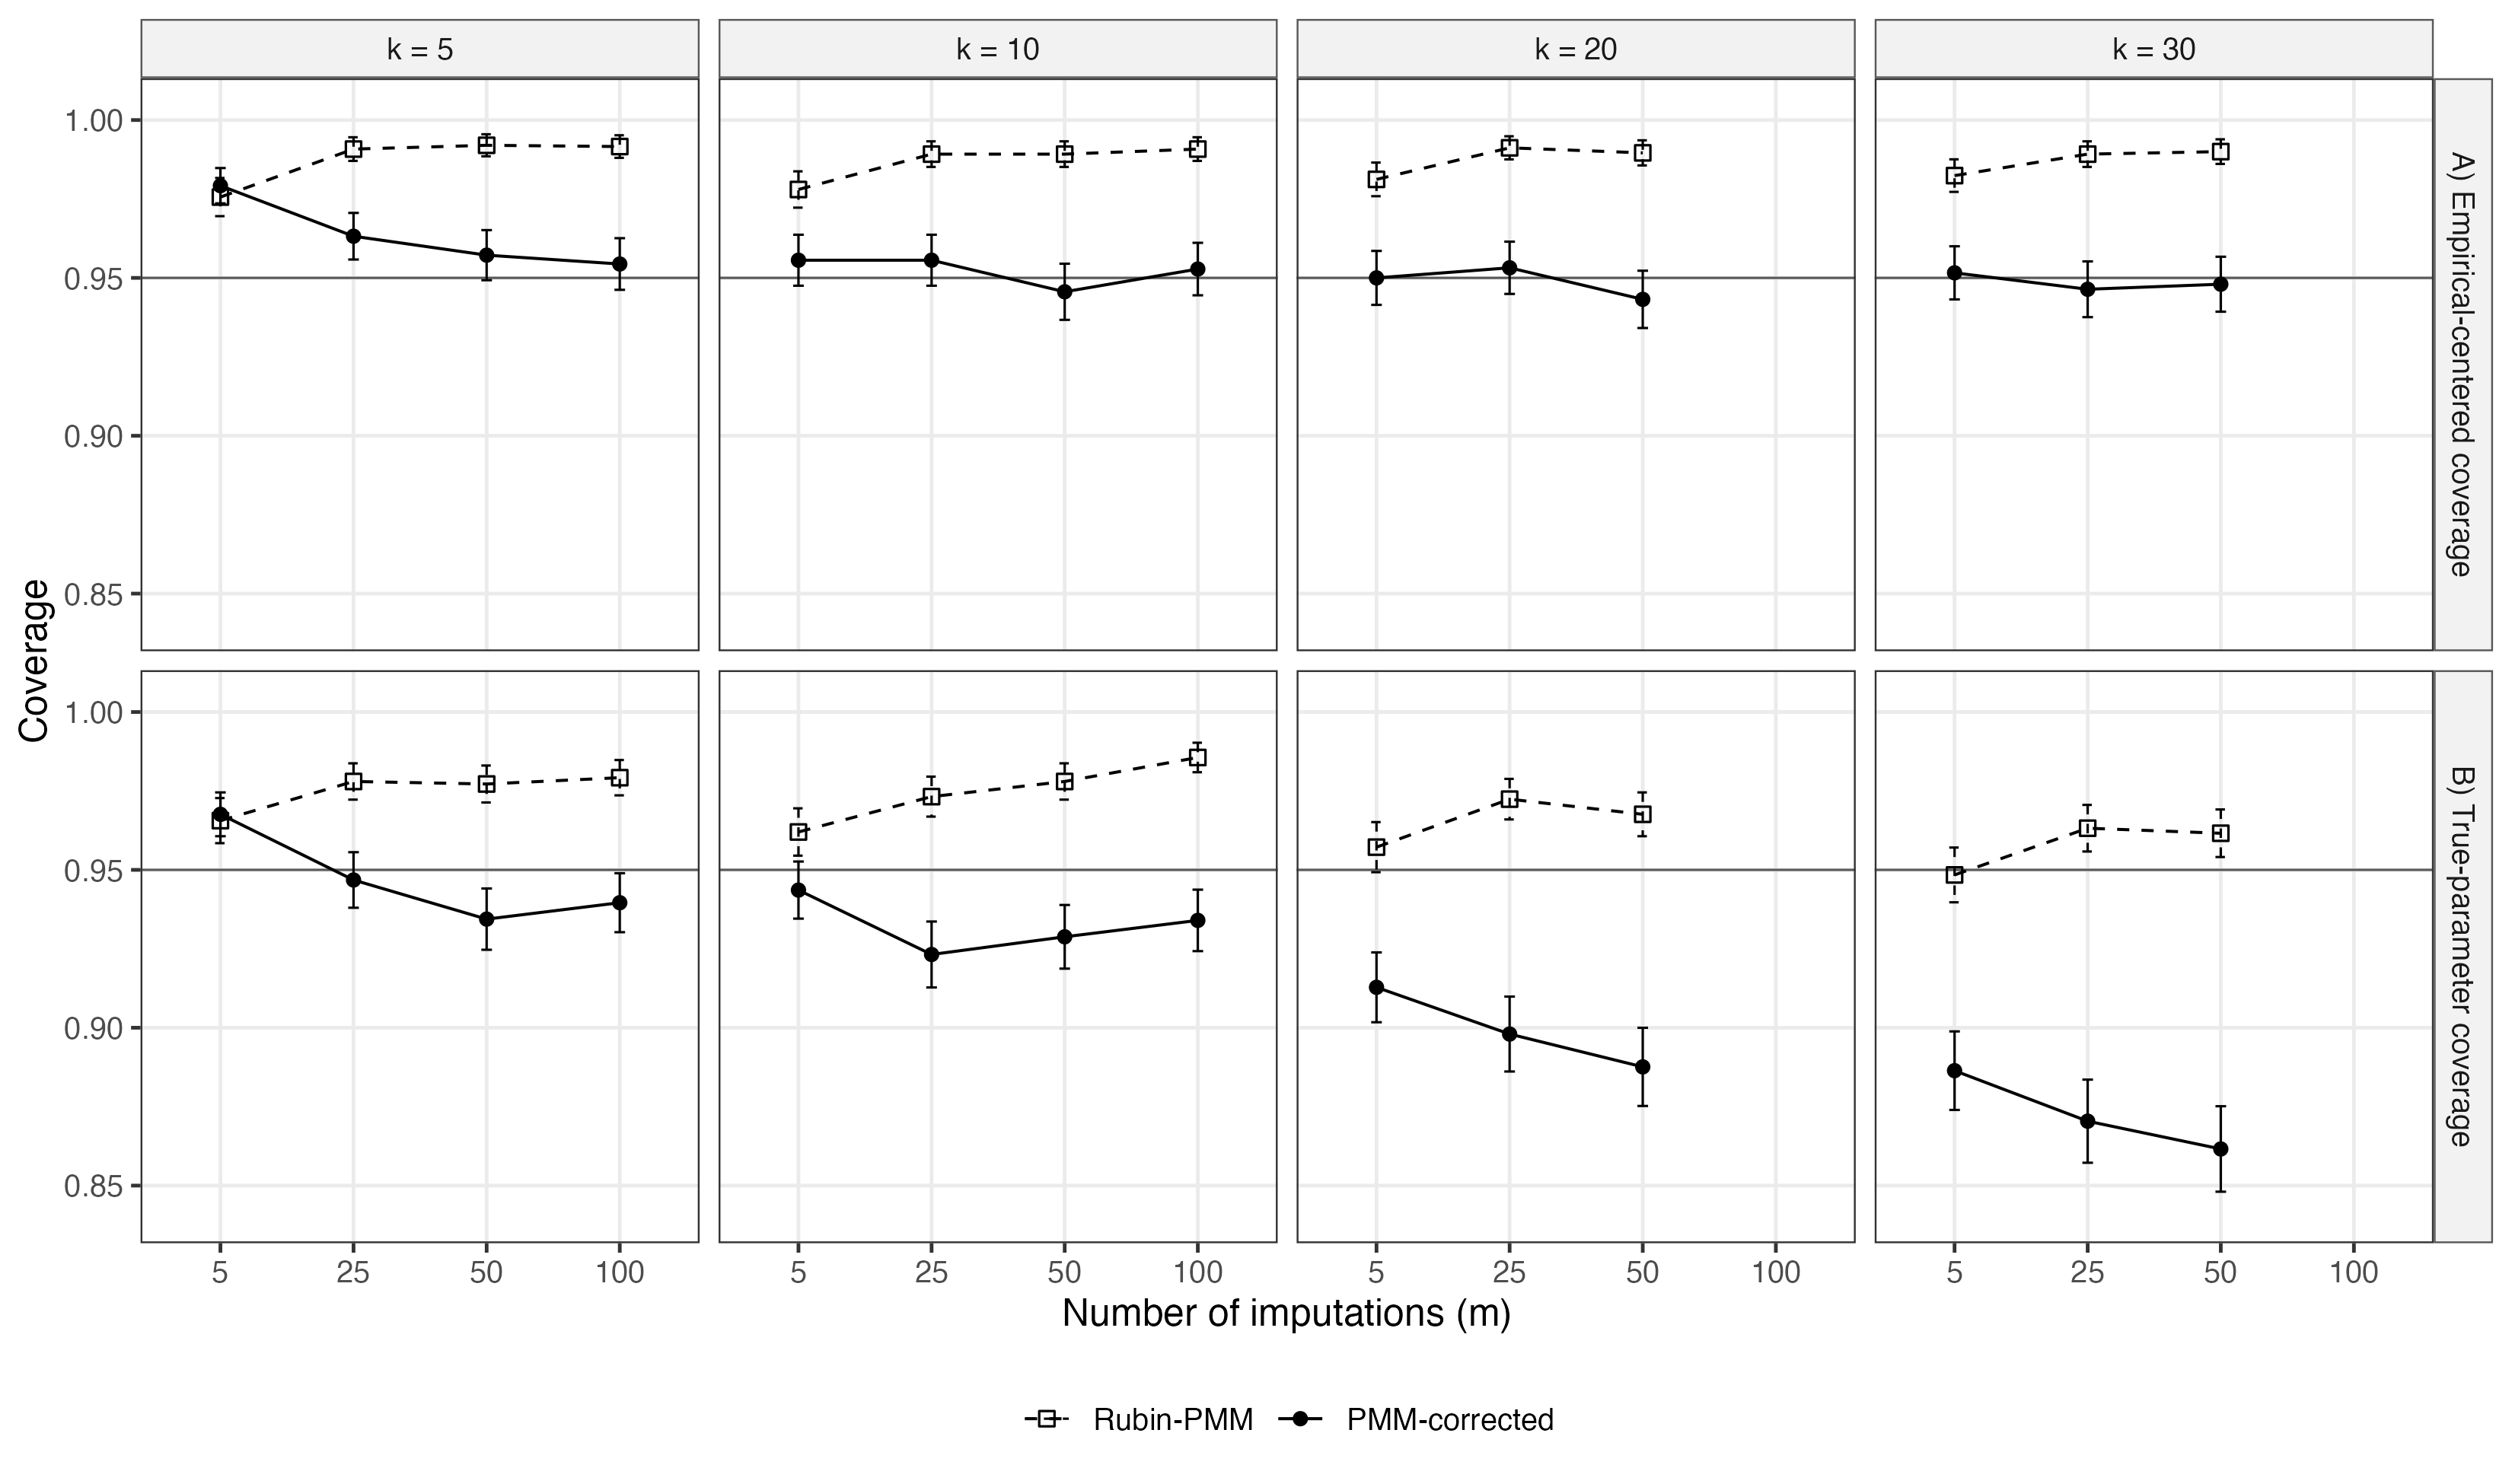
\includegraphics[width=\textwidth]{figures/gs_pmm_current_coverage_n2000.png}
\caption{RW-PMM measurement-error validation results at
\(n=2000\), shown across donor-width scales \(k\).  Rows distinguish
coverage of \(\beta^\ast\) from coverage of \(\beta_0\).  Empty points
mark simulation cells not included in the present result set.}
\label{fig:gs-pmm-current-n2000-supp}
\end{figure}
Figure~\ref{fig:gs-pmm-current-k5-supp} shows the available
RW-PMM validation cells graphically for donor-width scale
\(k=5\) across sample sizes.  Only cells with complete 2500-replicate
results are plotted.
\begin{figure}[ht]
\centering
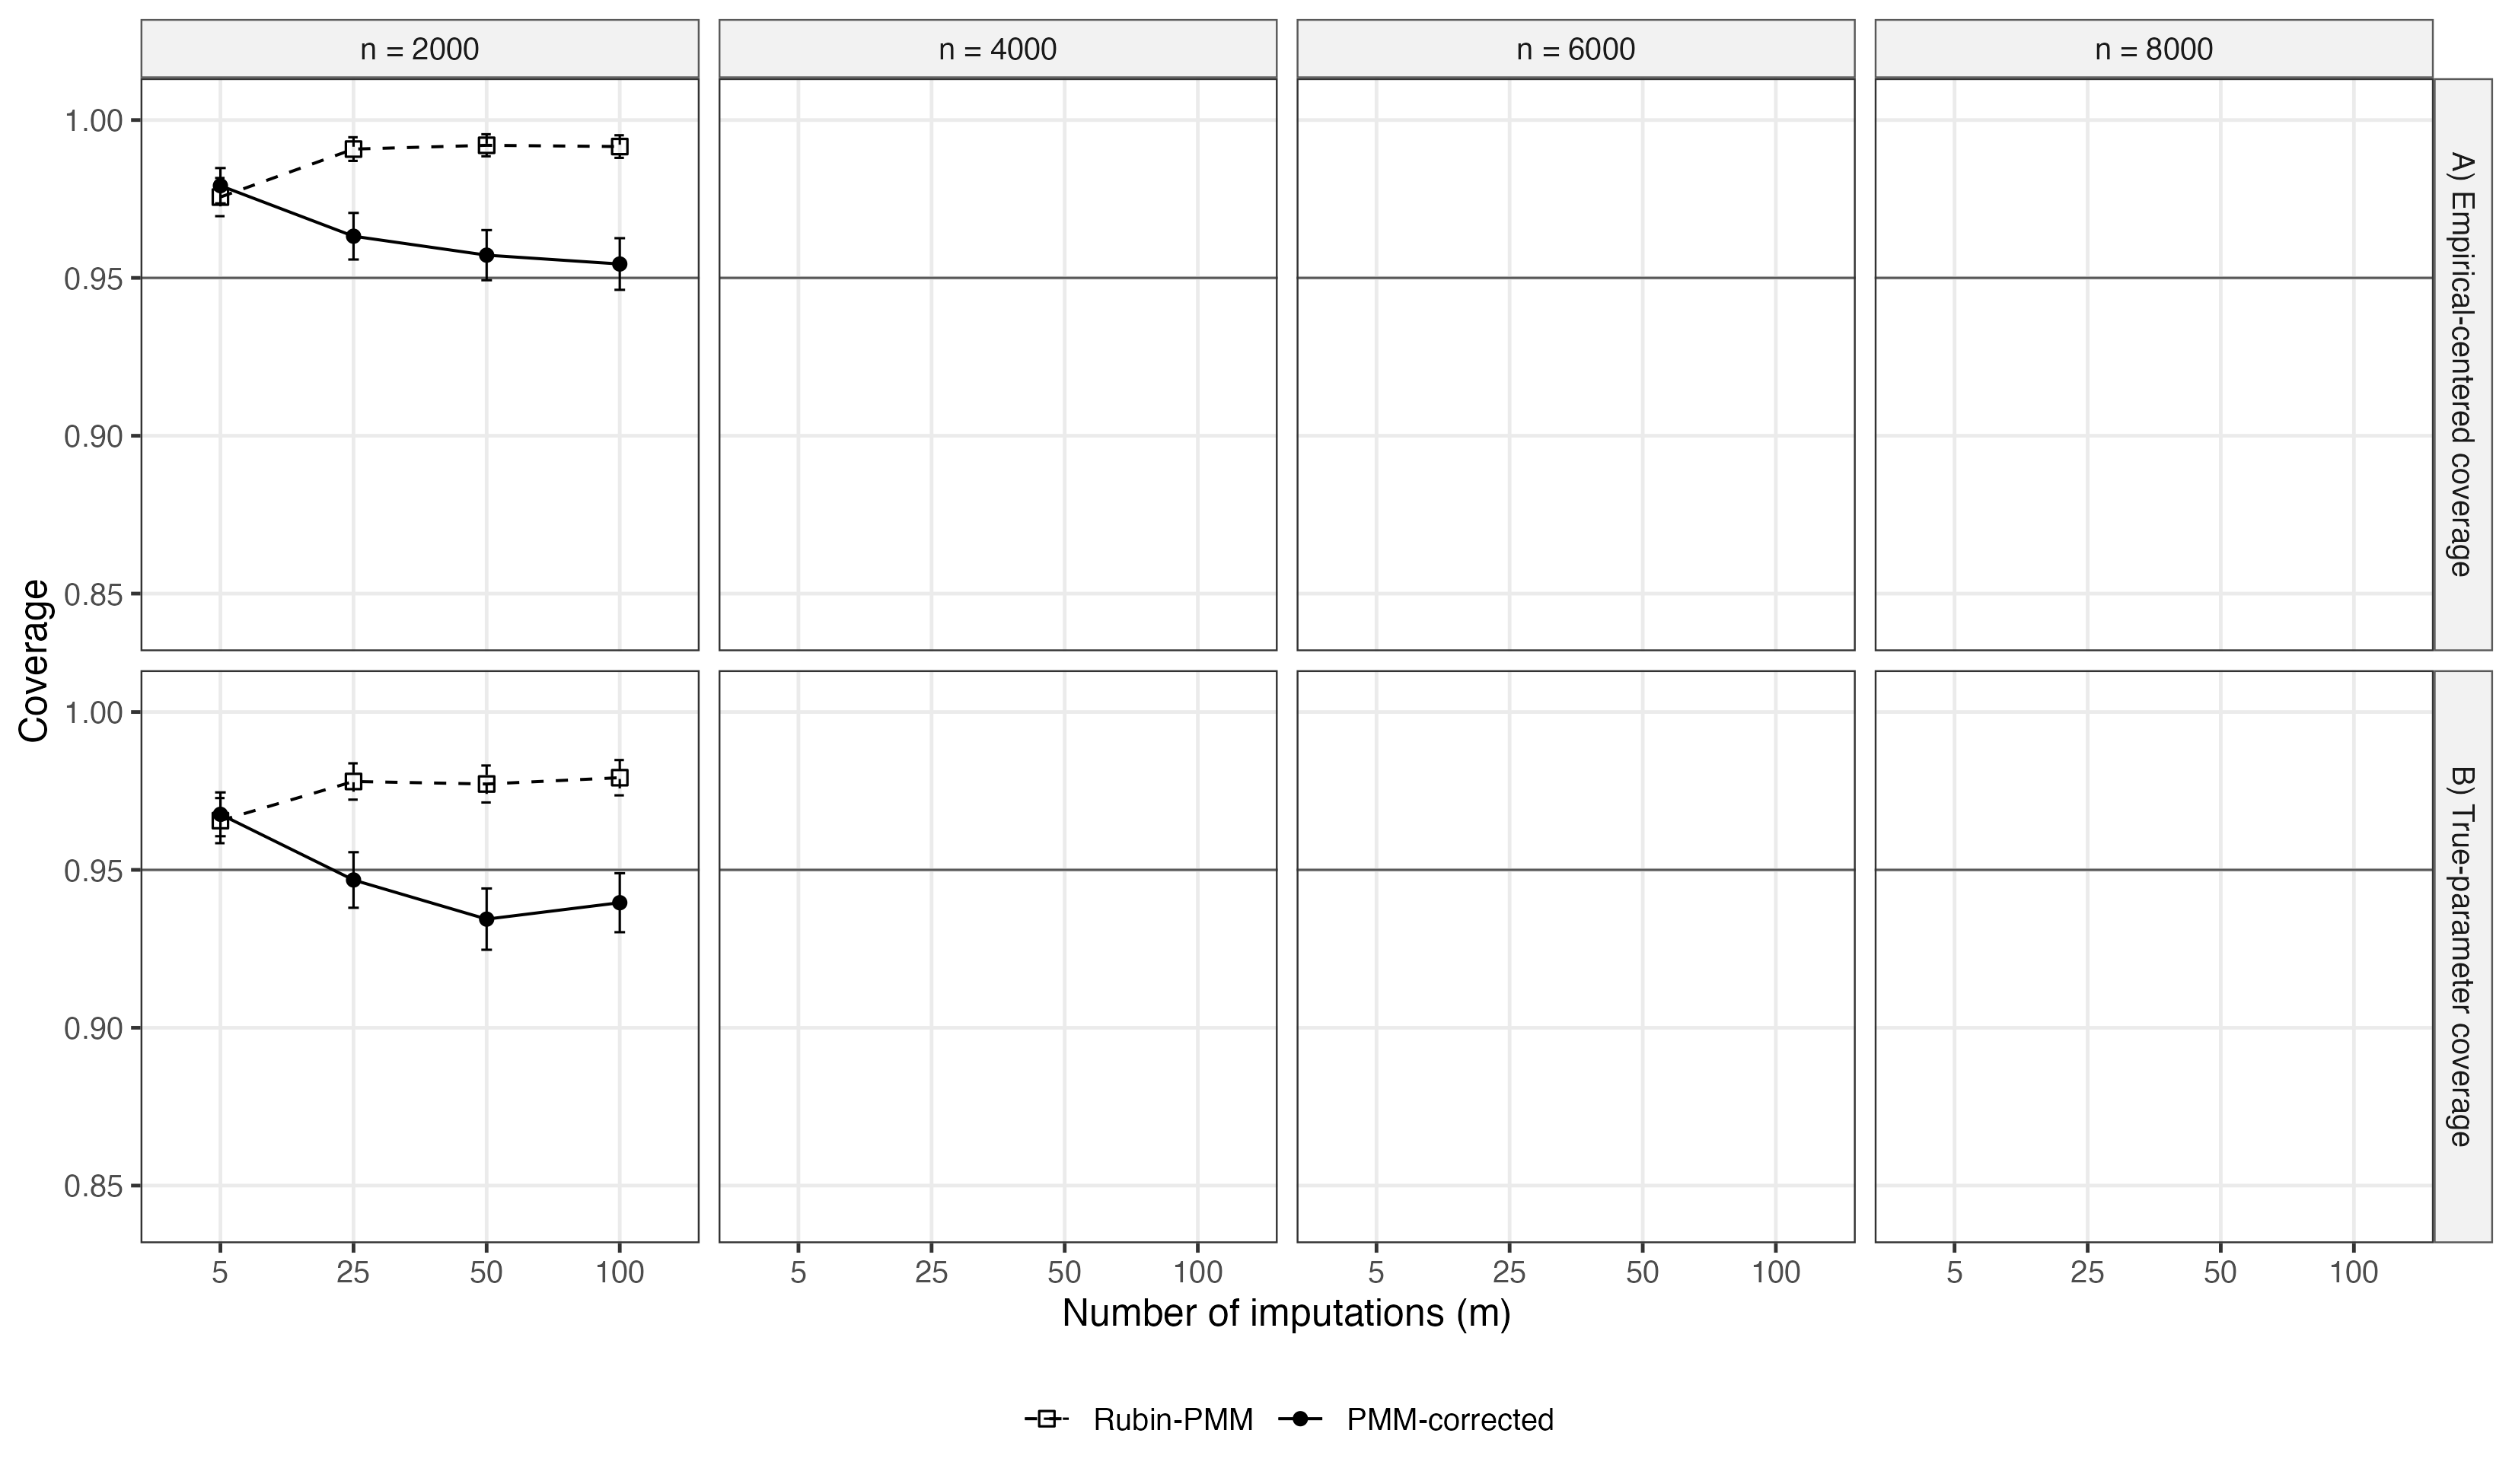
\includegraphics[width=\textwidth]{figures/gs_pmm_current_coverage_k5_by_n.png}
\caption{RW-PMM measurement-error validation results
for donor-width scale \(k=5\).  Columns show sample size \(n\), and
rows distinguish coverage of \(\beta^\ast\) from coverage of
\(\beta_0\).  Empty panels mark simulation cells not included in the
present result set.}
\label{fig:gs-pmm-current-k5-supp}
\end{figure}
For the parametric validation analysis, the main text focuses on the
original Giganti--Shepherd sample size \(n=4000\).
Figure~\ref{fig:gs-parametric-full-supp} shows the full parametric
measurement-error grid for \(n\in\{2000,4000,6000,8000\}\), which is
summarized in the main text only at \(n=4000\).
\begin{figure}[ht]
\centering
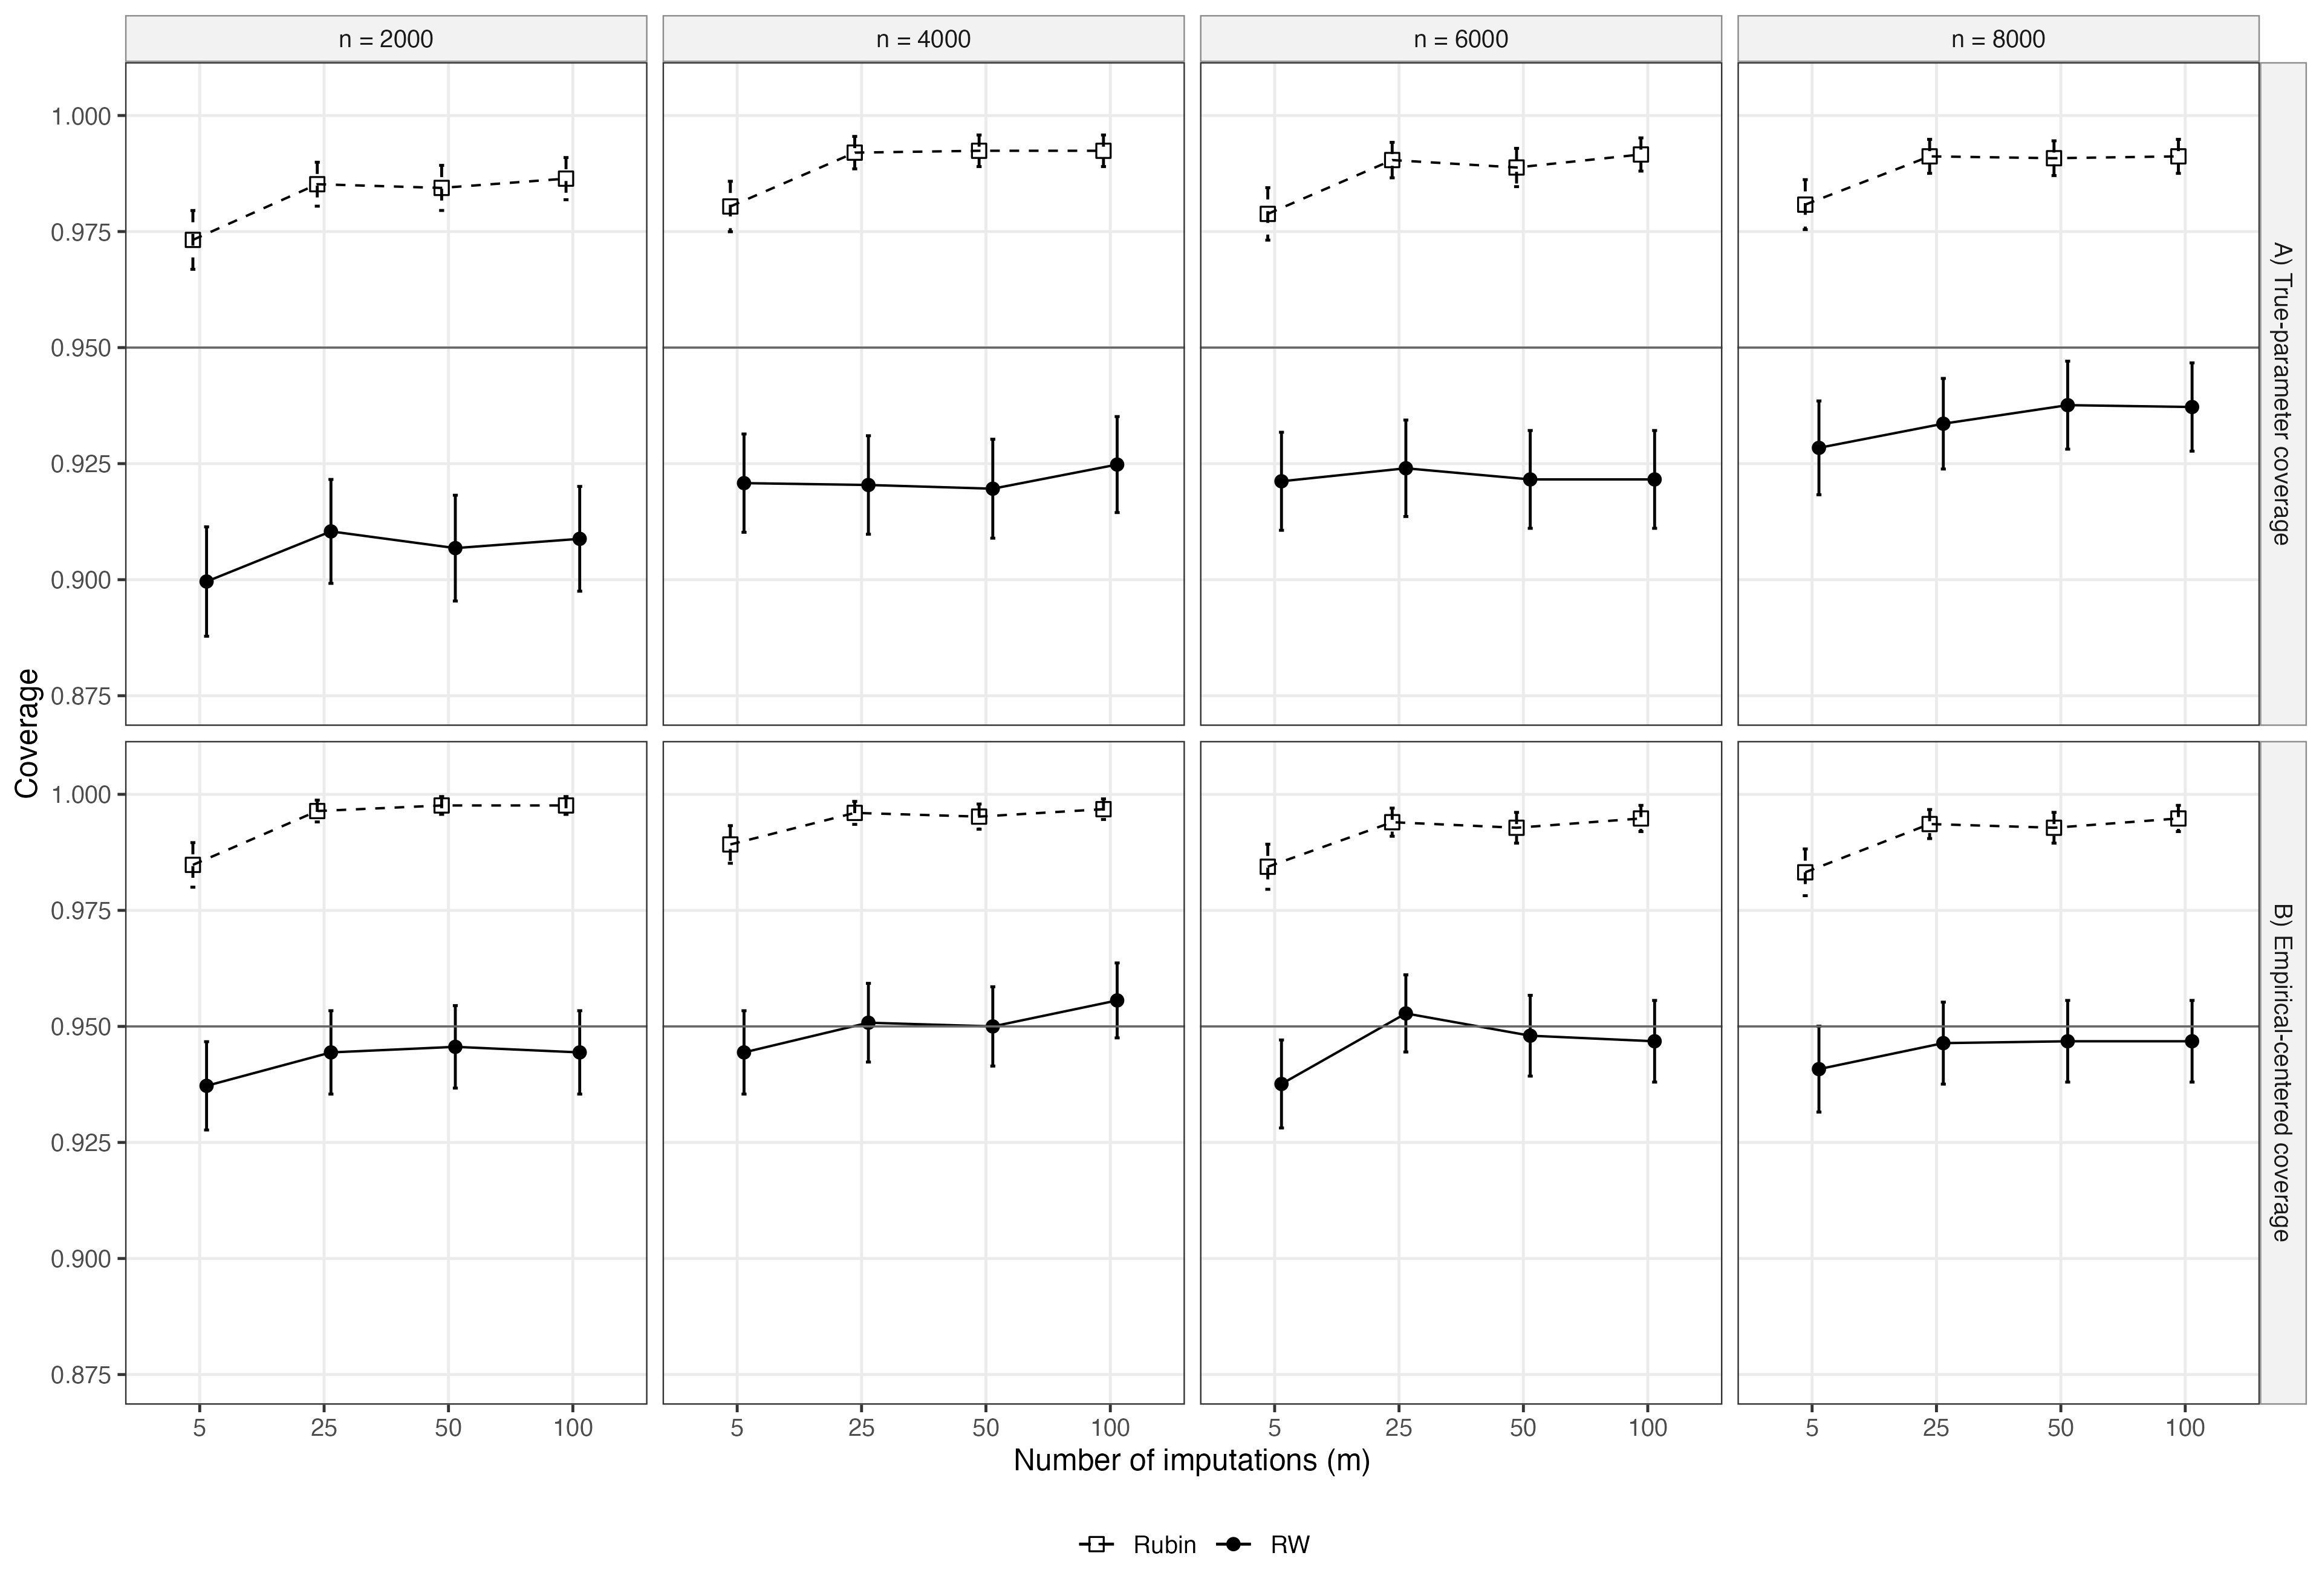
\includegraphics[width=\textwidth]{figures/gs_parametric_coverage.png}
\caption{Full parametric MICE measurement-error simulation grid. Rows
show coverage of \(\beta_0\) and coverage of \(\beta^\ast\) for the
chained conditional MICE implementation. The main text focuses on
\(n=4000\), matching the original Giganti--Shepherd sample size.}
\label{fig:gs-parametric-full-supp}
\end{figure}
\clearpage

\bibliography{papers}


\end{document}